\documentclass{beamer}
%kdfj
\usetheme[secheader]{Boadilla}
\setbeamertemplate{footline} {
  %\leavevmode%
  \hbox{%
  \begin{beamercolorbox}[wd=.5\paperwidth,ht=2.25ex,dp=1ex,left]{author in head/foot}%
    \usebeamerfont{author in head/foot}\hspace*{2ex}\insertshortauthor~~(adraeger@cern.ch)
  \end{beamercolorbox}%
  \begin{beamercolorbox}[wd=.5\paperwidth,ht=2.25ex,dp=1ex,right]{date in head/foot}%
    \usebeamerfont{date in head/foot}\insertshorttitle,~
    \insertshortdate{}\hspace*{1em}
    \insertframenumber{} / \inserttotalframenumber\hspace*{2ex}
  \end{beamercolorbox}}%
  \vskip0pt%
}
\beamertemplatenavigationsymbolsempty

\usepackage[percent]{overpic}
\usepackage{tikz}
%\usetikzlibrary{positioning,fit,shapes.arrows,shapes.geometric,shapes.misc,shapes.multipart,calc,shadows}
\tikzstyle{every picture}+=[remember picture]
\usepackage{booktabs}
\usepackage{graphicx}
\usepackage{rotating}
\usepackage{wasysym}
\usepackage{marvosym}
\usepackage{amssymb}
\usepackage{xcolor}
\usepackage{tabularx}
\usepackage[normalem]{ulem}
\graphicspath{{../../logo/}{figures/}{../../graphic-common/}}

\input{definitions.tex}
\newcommand{\lib}[1]{\tiny #1}

% Title etc
\vskip3cm
\title[Inclusive SUSY meeting]{Parametrization of Lepton \& Isolated Track Efficiencies \& Validation Using a Tag\&Probe Method}
\vskip3cm
\author[Arne-Rasmus~Dr\"ager]{
  Arne-Rasmus~Dr\"ager (University of Hamburg)\\ on behalf of the RA2/b team
}
\date[July 10, 2015]{July 10, 2015
%   \vskip1cm
  \begin{center}
    \includegraphics[height=1.5cm]{Universitaet-Hamburg-Logo.jpg}
    \hskip8cm
    \includegraphics[height=1.5cm]{CMSlogo.jpeg}
  \end{center}
}

% pdflatex packages
\hypersetup{bookmarks=true}
\hypersetup{unicode=false}
\hypersetup{pdftitle={Lost-Lepton}}
\hypersetup{pdfauthor={Arne-Rasmus~Dr\"ager}}


\begin{document}
% ==================================================
% --------------------------------------------------
\begin{frame}
  \titlepage
\end{frame}
\section{Introduction}
\begin{frame}
 \begin{overpic}[width=.32\textwidth]{figures/feynmanDiagrams/T1qqqq.pdf} \end{overpic}
 \begin{overpic}[width=.32\textwidth]{figures/feynmanDiagrams/T1tttt.pdf} \end{overpic}
 \begin{overpic}[width=.32\textwidth]{figures/feynmanDiagrams/T1bbbb_feyn.pdf} \end{overpic}\\
 \begin{itemize}
  \item RA2/b: Inclusive hadronic analyses targeting gluino production
  \begin{block}{}
  \begin{itemize}
   \item $\HT = \sum_{i}^{\text{jets}} |\vec{p_{T}},i| >500 \gev$ (jets: $\pt>30\gev$, $|\eta|<2.5$)
   \item $\MHT = |-\sum_{i}^{\text{jets}} \vec{p_{T}},i| >200 \gev$ (jets: $\pt>30\gev$, $|\eta|<5.0$)
   \item $\NJets\ge 4$ %(Jets: $\pt>30\gev$, $|\eta|<2.5$)
   \item $\BTags$= {$0,1,2,\geq3$} %(Jets: $\pt>30\gev$, $|\eta|<2.5$)
      \item $\Delta\phi_{1,2,3}>0.5,0.5,0.3$ (three leading jets)
   \item Veto: $\mu, e$ (mini isolation $\pt>10\gev, |\eta|<2.4(2.5)$)
   \item Veto: $\mu, e, \pi$ tracks ($\mu,e$: $\pt>5\gev$, $\pi$: $\pt>10\gev$)

  \end{itemize}
  \end{block}
  \item Split up baseline 72 exclusive search bins: \HT, \MHT, \NJets \& \BTags
 \end{itemize}
\end{frame}

\begin{frame}
 \frametitle{\ttbar, \wpj \& Single t Event Rejection Strategy}
 \begin{columns}
  \begin{column}{0.6\textwidth}
   \begin{itemize}
    \item Veto events with
    \begin{itemize}
     \item Isolated $e,\mu$
     \item Isolated $e,\mu,\pi$ tracks
    \end{itemize}
\item Isolated $\mu$, e:
 \begin{itemize}
  \item $\pt>10 \gev, |\eta|<2.4(2.5)$
  \item "Tight"ID (WP "veto")
  \item $I_{mini}<0.2(0.1)$
 \end{itemize}
   \end{itemize}
  \end{column}
  \begin{column}{0.4\textwidth}
\begin{tikzpicture}
    \node[anchor=south west,inner sep=0] (image) at (0,0) {\includegraphics[width=0.75\textwidth]{figures/Sketches/Wpjsketch.png}};
    \begin{scope}[x={(image.south east)},y={(image.north west)}]
%         \draw[red,ultra thick,rounded corners] (0.62,0.65) rectangle (0.78,0.75);
%         \draw[red,ultra thick,rounded corners] (0.60,0.01) rectangle (0.75,0.99); % coordinates unten links(x,y) oben rechts(x,y)
%             \draw[blue,ultra thick,rounded corners] (0.40,0.01) rectangle (0.55,0.99); % coordinates unten links(x,y) oben rechts(x,y)
    \end{scope}
\end{tikzpicture}   
\begin{tikzpicture}
    \node[anchor=south west,inner sep=0] (image) at (0,0) {\includegraphics[width=0.75\textwidth]{figures/Sketches/miniIso.png}};
    \begin{scope}[x={(image.south east)},y={(image.north west)}]
%         \draw[red,ultra thick,rounded corners] (0.62,0.65) rectangle (0.78,0.75);
%         \draw[red,ultra thick,rounded corners] (0.60,0.01) rectangle (0.75,0.99); % coordinates unten links(x,y) oben rechts(x,y)
%             \draw[blue,ultra thick,rounded corners] (0.40,0.01) rectangle (0.55,0.99); % coordinates unten links(x,y) oben rechts(x,y)
    \end{scope}
\end{tikzpicture}  
  \end{column}
 \end{columns}
 \begin{itemize}
    \item Isolated $\mu,e$ tracks:
 \begin{itemize}
  \item Charged PFCand, $\pt>5 \gev, |\eta|<2.5$, $\mt<100 \gev$, pdgID=11,13
  \item Iso: $\Sigma ( \pt\text(Tracks)\Delta R<0.3 )/(\pt Track) < 0.2$ (with $dz<0.1$)
 \end{itemize}
 \item Isolated $\pi$ tracks:
 \begin{itemize}
  \item Charged PFCand, $\pt>10 \gev, |\eta|<2.5$, $\mt<100 \gev$, pdgID=211
  \item Iso: $\Sigma ( \pt\text(Tracks)\Delta R<0.3 )/(\pt Track) < 0.1$ (with $dz<0.1$)
 \end{itemize}
%   \item show here feynmanDiagrams of ttbar wpj for illustration maybe also the other backgrounds
%   \item Important to note that we have two handles on reducing the \ttbar \wpj single top background due to non detected $e\mu$
%   \item Explicit isolated $\mu, e$ reduce \ttbar \wpj background
%   \item In addition \& $\mu, e, \pi$ track veto rejects
 \end{itemize}
 \begin{block}{}
 \centering
 \underline{Two handles on rejecting $\mu,e$ events!!}
 \end{block}
\end{frame}

\section{$\mu,e$ Efficiencies}
\begin{frame}
 \begin{block}{}
 \centering
 \Large $\mu,e$ Efficiencies
 \end{block}
\end{frame}


\subsection{Lost-Lepton Method}
\begin{frame}
\frametitle{Concept: Estimating Lost $e,\mu$ from \wpj \& \ttbar Events}
 \begin{center}
\begin{tikzpicture}
    \node[anchor=south west,inner sep=0] (image) at (0,0) {\includegraphics[width=0.75\textwidth]{figures/Sketches/LostLeptonSketch_mu_pred.png}};
    \begin{scope}[x={(image.south east)},y={(image.north west)}]
%         \draw[red,ultra thick,rounded corners] (0.62,0.65) rectangle (0.78,0.75);
%         \draw[red,ultra thick,rounded corners] (0.60,0.01) rectangle (0.75,0.99); % coordinates unten links(x,y) oben rechts(x,y)
%             \draw[blue,ultra thick,rounded corners] (0.40,0.01) rectangle (0.55,0.99); % coordinates unten links(x,y) oben rechts(x,y)
    \end{scope}
\end{tikzpicture}
 \end{center}
  \begin{itemize}
  \item Select control sample (CS): Exactly one well isolated $e/\mu$ within acceptance cuts
  \item Weight each CS event according to inefficiencies for each identification step
 \end{itemize}
\end{frame}
\subsection{Parametrization of Efficiencies}
\begin{frame}
 \frametitle{Expected Control-Sample Events (4$\fb^{-1}$)}
\begin{columns}
  \begin{column}{0.6\textwidth}
  \begin{tikzpicture}
    \node[anchor=south west,inner sep=0] (image) at (0,0) {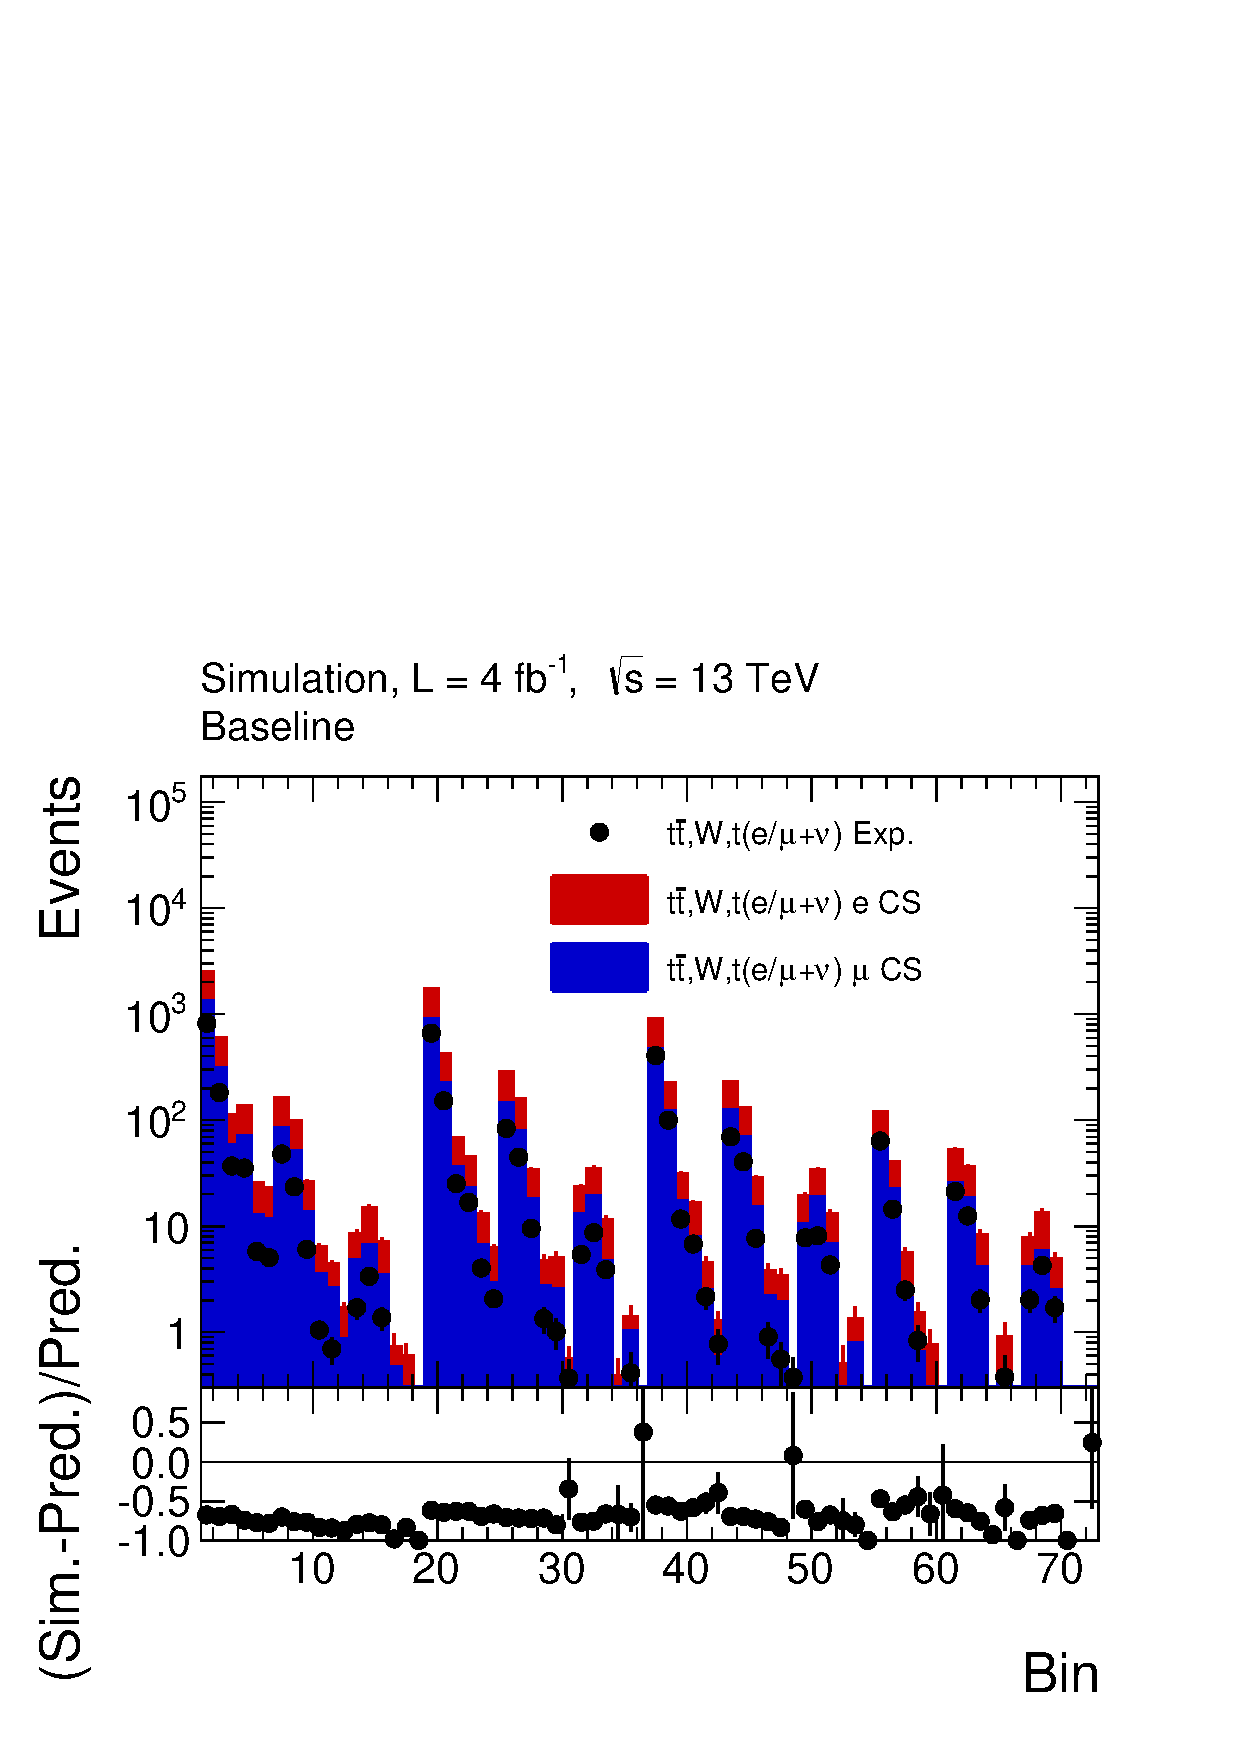
\includegraphics[width=0.90\textwidth]{figures/lost-lepton/CS_VS_Expectation/Baseline/CS_VS_Expectation__Bin__MCExTotal_vs_MCMuCS+MCElecCS__Baseline.pdf}};
    \begin{scope}[x={(image.south east)},y={(image.north west)}]
%         \draw[red,ultra thick,rounded corners] (0.62,0.65) rectangle (0.78,0.75);
%         \draw[red,ultra thick,rounded corners] (0.60,0.01) rectangle (0.75,0.99); % coordinates unten links(x,y) oben rechts(x,y)
%             \draw[blue,ultra thick,rounded corners] (0.40,0.01) rectangle (0.55,0.99); % coordinates unten links(x,y) oben rechts(x,y)
    \end{scope}
\end{tikzpicture}   
  \end{column}
  \begin{column}{0.4\textwidth}
  \begin{center}
     \begin{tikzpicture}
    \node[anchor=south west,inner sep=0] (image) at (0,0) {\includegraphics[width=0.60\textwidth]{figures/Sketches/BinsBox.png}};
    \begin{scope}[x={(image.south east)},y={(image.north west)}]
%         \draw[red,ultra thick,rounded corners] (0.62,0.65) rectangle (0.78,0.75);
%         \draw[red,ultra thick,rounded corners] (0.60,0.01) rectangle (0.75,0.99); % coordinates unten links(x,y) oben rechts(x,y)
%             \draw[blue,ultra thick,rounded corners] (0.40,0.01) rectangle (0.55,0.99); % coordinates unten links(x,y) oben rechts(x,y)
    \end{scope}
\end{tikzpicture}
   
  \end{center}
 
   \tiny Binning:\\
   \tiny Bin 1-6: $4\leq\NJets\leq6, \BTags=0$\\
   \tiny Bin 7-12: $4\leq\NJets\leq6, \BTags=1$ etc.\\
   \tiny Bin 25-31: $7\leq\NJets\leq8, \BTags=0$ etc.\\
  \end{column}
 \end{columns}
    \begin{itemize}
    \item Expect low statistics in some exclusive search bins.
    \item Event MC lags of statistics in some bins (can not derive eff. for each search bin)
   \end{itemize}
\end{frame}
% \subsection{Efficiency Parametrization}
\begin{frame}
 \frametitle{Region with little expected CS events}
 \begin{itemize}
  \item Most sensitive search regions contain few $e/\mu$ control-sample events
  \item Important: \underline{Choice of efficiency parametrization!}
  \item Different approaches:
  \begin{itemize}
   \item 1. Event topology based parametrization,\\ eg. \pt lepton \deltaR lepton closest jet
   \item 2. Search bin based efficiencies: Binned in \HT, \MHT, \NJets \& \BTags
  \end{itemize}
 \end{itemize}
 \noindent\makebox[\linewidth]{\rule{\textwidth}{0.4pt}}
 \begin{columns}
  \begin{column}{0.465\textwidth}
  Option 1
   \begin{itemize}
    \item Can be obtained directly from data using a Tag \& Probe method
    \item Difficult to parametrize event topology independent: Obtain from \Zll apply to \ttbar \wpj events
   \end{itemize}

  \end{column}
  \begin{column}{0.535\textwidth}
     Option 2
   \begin{itemize}
    \item Can not be obtained from data, validated indirectly via Tag\&Probe
    \item Captures \ttbar \& \wpj event kinematics according to simulation quality
    \item Lags of statistics (exclusive search bins)
   \end{itemize}
  \end{column}

 \end{columns}
\end{frame}
\begin{frame}
\frametitle{Closer look at option 1}
    \begin{itemize}
   \item Classical approach of lepton \pt, jet \pt \& $\Delta R$ shows strong variation of efficiency and is strongly correlated with lepton isolation definition
   \item Severe problem when applying method to low statistical regions!
  \end{itemize}
  \begin{columns}
   \begin{column}{0.45\textwidth}
   \centering
%     \small  Typical $\mu$ isolation efficiency
    \begin{overpic}[width=.99\textwidth]{figures/efficiencies/MuIsoDeltaRRelPTJet.pdf}
    \end{overpic}
   \end{column}
  \begin{column}{0.55\textwidth}
   Example: Region with 3 gen 1 CS event\\
    \begin{overpic} [width=0.45\textwidth]{figures/Sketches/deltaRLowStat.pdf}
      \end{overpic}
      \begin{overpic} [width=0.45\textwidth]{figures/Sketches/deltaRLowStatReco.pdf}
      \end{overpic}
     
  \end{column}
  \end{columns}
  \begin{itemize}
   \item Strong variation of efficiencies ($10-99\%$) lead to large fluctuations in low statistics regions
   \item Need to find parametrization:
   \begin{itemize}
    \item Capture event based topology in order to make transfer\\ \Zll to \ttbar, \wpj event kinematics
    \item Less dependent to avoid large fluctuations
   \end{itemize}
  \end{itemize}
\end{frame}

\begin{frame}
 \frametitle{Motivation: Activity}
 \begin{itemize}
  \item Combine lepton \pt with subset of activity around the lepton in a fixed large cone size ($R=1.0$)
  \begin{itemize}
\item Not orthogonal but also not fully correlated to isolation definition $\rightarrow$ subset of energy in cone around lepton
 \item Capture event kinematics in a more broader frame 'averaging' over range of strong efficiency drop in $\Delta R$
  \end{itemize}
 \end{itemize}
 
   \begin{columns}
   \begin{column}{0.5\textwidth}
   \centering
   \small $\Delta R$ \& lepton \pt / jet \pt
    \begin{overpic}[width=.99\textwidth]{figures/efficiencies/MuIsoDeltaRRelPTJet.pdf}
    \end{overpic}
   \end{column}
  \begin{column}{0.5\textwidth}
   \centering
    \small  lepton \pt, activity
    \begin{overpic}[width=.99\textwidth]{figures/efficiencies/MuIsoPTActivity.pdf}
%            \put(63,61.5){\rotatebox{-0}{\scriptsize Work in progress}}
    \end{overpic}
     
  \end{column}
  \end{columns}
\end{frame}




\begin{frame}
 \frametitle{Activity Definition \& Comparison}
  \begin{itemize}
  \item Muon: $A = \sum_{Jet}^{\Delta R<1.0} \pt(Jet) * (ChargedEMFrac + ChargedHadFrac) $
    \item Electron: $A = \sum_{Jet}^{\Delta R<1.0} \pt(Jet) * (ChargedHadFrac) $
  \end{itemize}
\begin{columns}
  \begin{column}{0.5\textwidth}
  \centering
   \small $\Delta R$ \& lepton \pt / jet \pt
\begin{tikzpicture}
    \node[anchor=south west,inner sep=0] (image) at (0,0) {\includegraphics[width=0.90\textwidth]{figures/efficiencies/MuIsoDeltaRRelPTJet.pdf}};
    \begin{scope}[x={(image.south east)},y={(image.north west)}]
%         \draw[red,ultra thick,rounded corners] (0.62,0.65) rectangle (0.78,0.75);
%         \draw[red,ultra thick,rounded corners] (0.60,0.01) rectangle (0.75,0.99); % coordinates unten links(x,y) oben rechts(x,y)
%             \draw[blue,ultra thick,rounded corners] (0.40,0.01) rectangle (0.55,0.99); % coordinates unten links(x,y) oben rechts(x,y)
    \end{scope}
\end{tikzpicture}  
  \end{column}
  \begin{column}{0.5\textwidth}
  \centering
      \small  lepton \pt, activity
\begin{tikzpicture}
    \node[anchor=south west,inner sep=0] (image) at (0,0) {\includegraphics[width=0.90\textwidth]{figures/efficiencies/MuIsoPTActivity.pdf}};
    \begin{scope}[x={(image.south east)},y={(image.north west)}]
%         \draw[red,ultra thick,rounded corners] (0.62,0.65) rectangle (0.78,0.75);
%         \draw[red,ultra thick,rounded corners] (0.60,0.01) rectangle (0.75,0.99); % coordinates unten links(x,y) oben rechts(x,y)
%             \draw[blue,ultra thick,rounded corners] (0.40,0.01) rectangle (0.55,0.99); % coordinates unten links(x,y) oben rechts(x,y)
    \end{scope}
\end{tikzpicture}   
  \end{column}
 \end{columns}
 \begin{itemize}
  \item $\Delta R:$ Steep drop towards low values $99\%\rightarrow 10\%$!
  \item Activity: Moderate dependency on activity ($99\%\rightarrow 74\%$)
 \end{itemize}
  \begin{block}{}
 \centering
 Is activity able to achieve good closure?\\ Parametrization independent of physics process?
 \end{block}
\end{frame}



\begin{frame}
 \frametitle{Closure Test: Non-Isolated $\mu$}
   \begin{columns}
       \begin{column}{0.45\textwidth}
       \begin{center}
     \begin{tikzpicture}
    \node[anchor=south west,inner sep=0] (image) at (0,0) {\includegraphics[width=0.80\textwidth]{figures/Sketches/PredictionIsoPartOnly.png}};
    \begin{scope}[x={(image.south east)},y={(image.north west)}]
%         \draw[red,ultra thick,rounded corners] (0.62,0.65) rectangle (0.78,0.75);
%         \draw[red,ultra thick,rounded corners] (0.60,0.01) rectangle (0.75,0.99); % coordinates unten links(x,y) oben rechts(x,y)
%             \draw[blue,ultra thick,rounded corners] (0.40,0.01) rectangle (0.55,0.99); % coordinates unten links(x,y) oben rechts(x,y)
    \end{scope}
\end{tikzpicture}       
       \end{center}
   \end{column}
       \begin{column}{0.55\textwidth}
       \begin{center}
    \begin{tikzpicture}
    \node[anchor=south west,inner sep=0] (image) at (0,0) {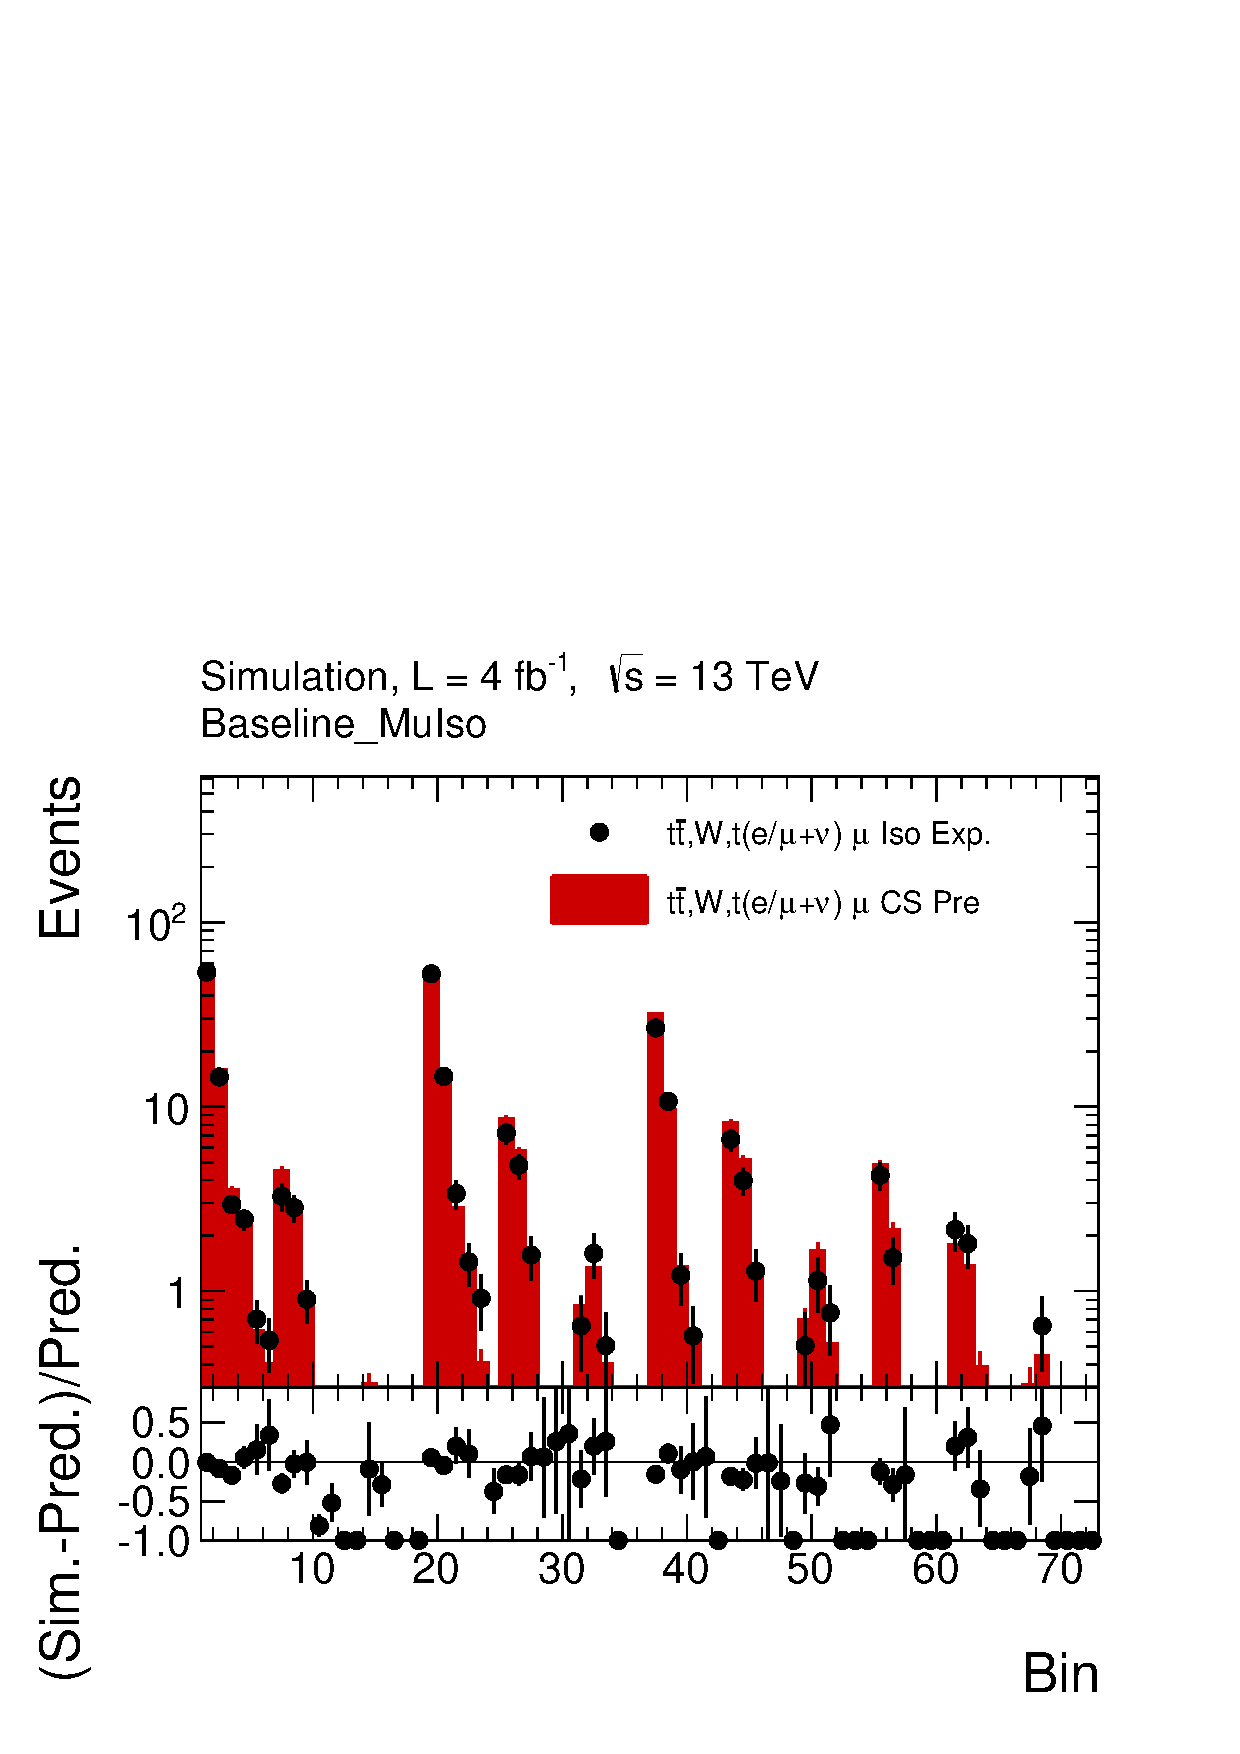
\includegraphics[width=0.90\textwidth]{figures/lost-lepton/Closure_Step_By_Step_Mu/Baseline_MuIso/Closure_Step_By_Step_Mu__Bin__MCEx_vs_MuCSMTWDiLepCorrected__Baseline_MuIso.pdf}};
    \begin{scope}[x={(image.south east)},y={(image.north west)}]
%         \draw[red,ultra thick,rounded corners] (0.62,0.65) rectangle (0.78,0.75);
%         \draw[red,ultra thick,rounded corners] (0.60,0.01) rectangle (0.75,0.99); % coordinates unten links(x,y) oben rechts(x,y)
%             \draw[blue,ultra thick,rounded corners] (0.40,0.01) rectangle (0.55,0.99); % coordinates unten links(x,y) oben rechts(x,y)
    \end{scope}
\end{tikzpicture}  
       \end{center}
   \end{column}
\end{columns}
%  \begin{columns}
%   \begin{column}{0.5\textwidth}
% \begin{tikzpicture}
%     \node[anchor=south west,inner sep=0] (image) at (0,0) {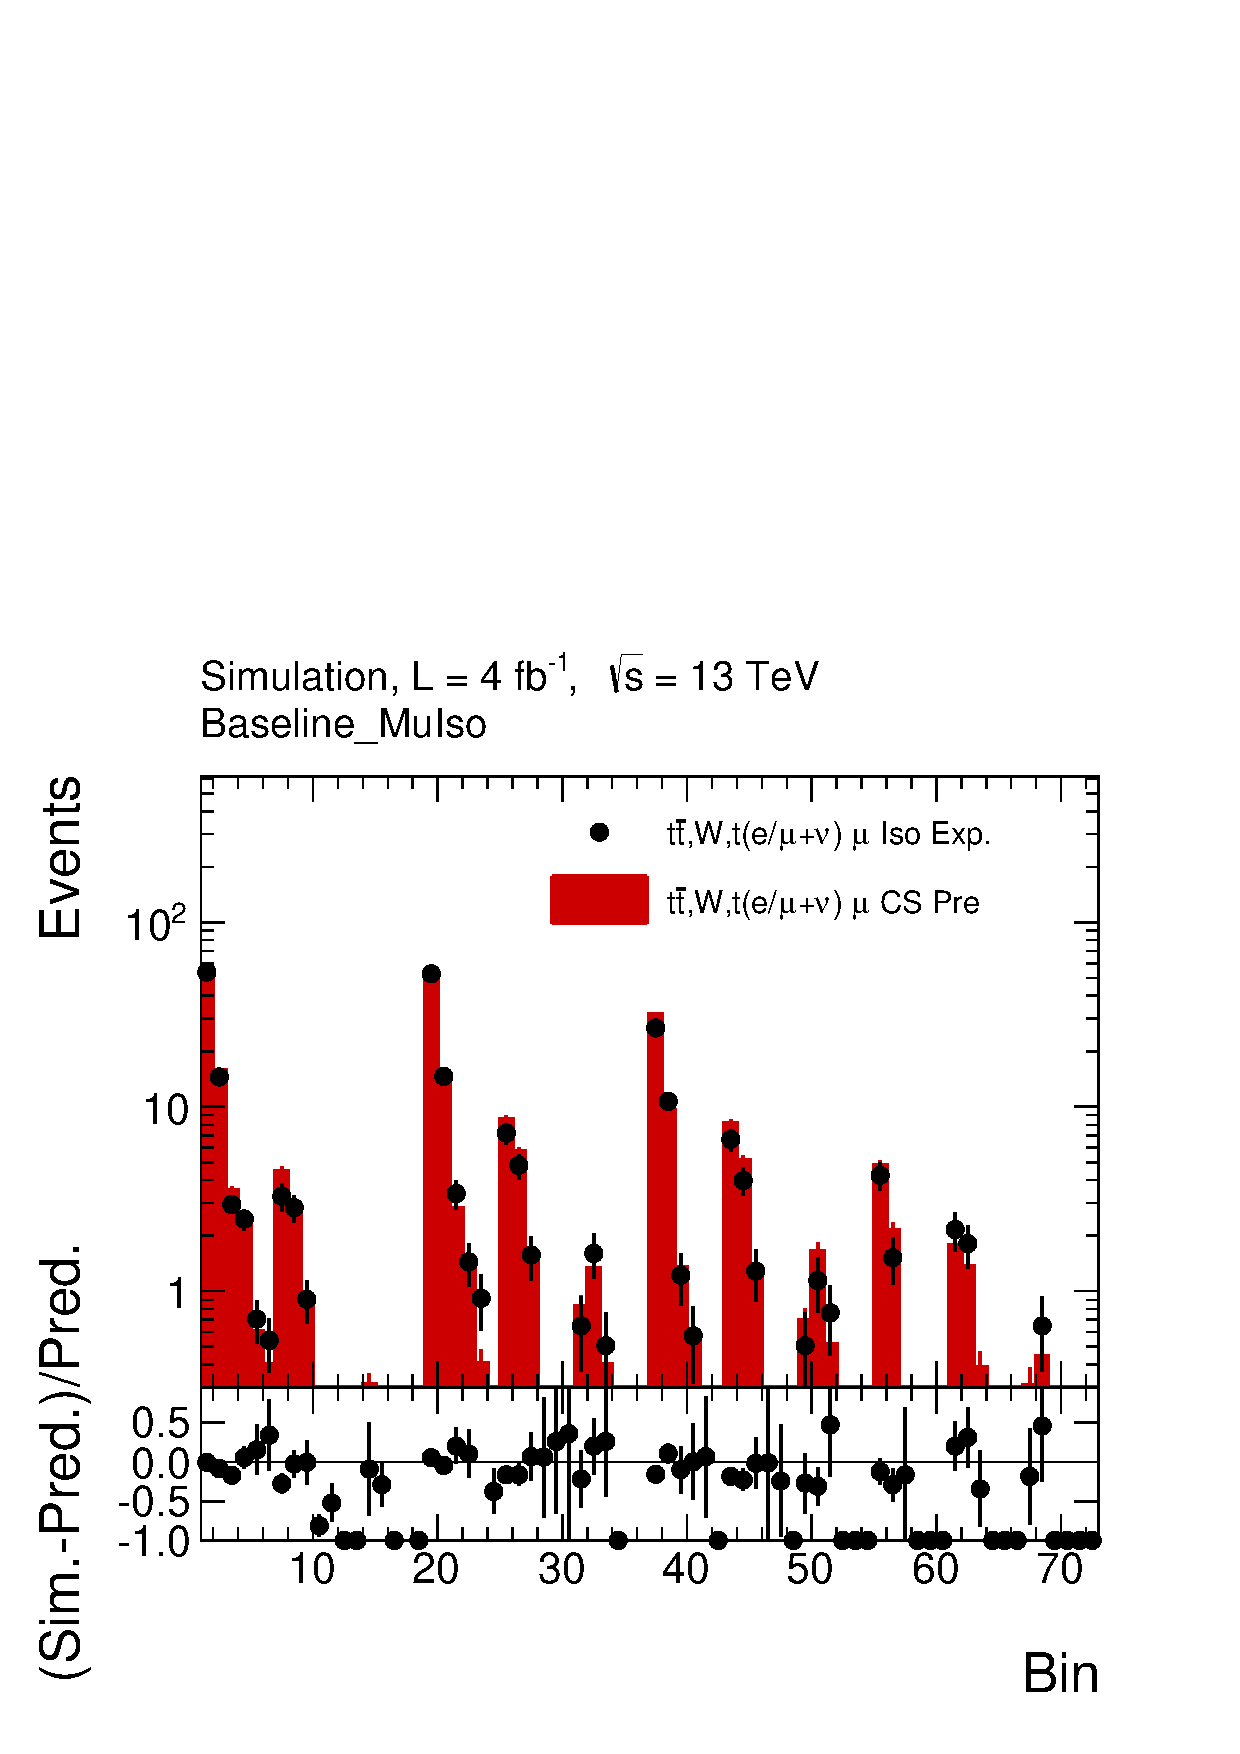
\includegraphics[width=0.90\textwidth]{figures/lost-lepton/Closure_Step_By_Step_Mu/Baseline_MuIso/Closure_Step_By_Step_Mu__Bin__MCEx_vs_MuCSMTWDiLepCorrected__Baseline_MuIso.pdf}};
%     \begin{scope}[x={(image.south east)},y={(image.north west)}]
% %         \draw[red,ultra thick,rounded corners] (0.62,0.65) rectangle (0.78,0.75);
% %         \draw[red,ultra thick,rounded corners] (0.60,0.01) rectangle (0.75,0.99); % coordinates unten links(x,y) oben rechts(x,y)
% %             \draw[blue,ultra thick,rounded corners] (0.40,0.01) rectangle (0.55,0.99); % coordinates unten links(x,y) oben rechts(x,y)
%     \end{scope}
% \end{tikzpicture}  
%   \end{column}
%   \begin{column}{0.5\textwidth}
% \begin{tikzpicture}
%     \node[anchor=south west,inner sep=0] (image) at (0,0) {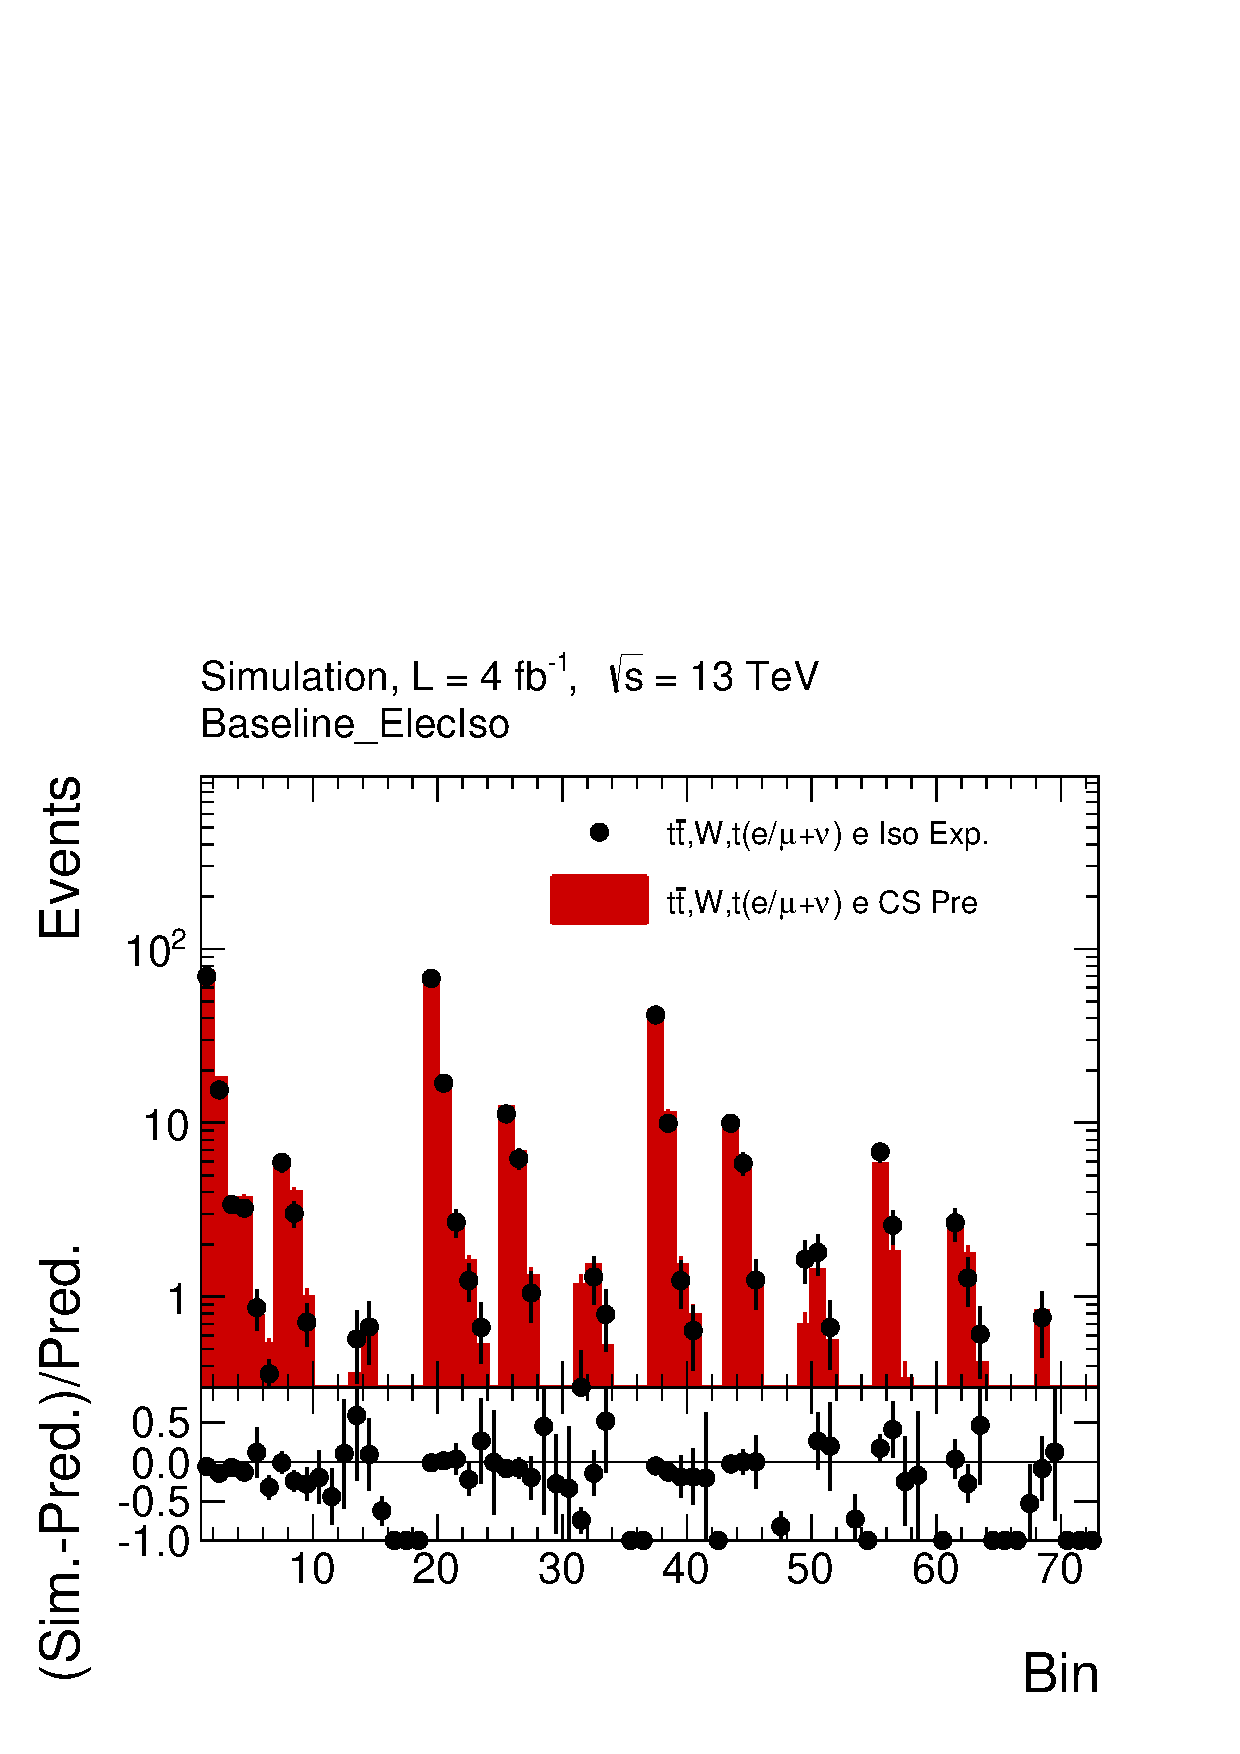
\includegraphics[width=0.90\textwidth]{figures/lost-lepton/Closure_Step_By_Step_Elec/Baseline_ElecIso/Closure_Step_By_Step_Elec__Bin__MCEx_vs_ElecCSMTWDiLepCorrected__Baseline_ElecIso.pdf}};
%     \begin{scope}[x={(image.south east)},y={(image.north west)}]
% %         \draw[red,ultra thick,rounded corners] (0.62,0.65) rectangle (0.78,0.75);
% %         \draw[red,ultra thick,rounded corners] (0.60,0.01) rectangle (0.75,0.99); % coordinates unten links(x,y) oben rechts(x,y)
% %             \draw[blue,ultra thick,rounded corners] (0.40,0.01) rectangle (0.55,0.99); % coordinates unten links(x,y) oben rechts(x,y)
%     \end{scope}
% \end{tikzpicture}   
%   \end{column}
%  \end{columns}
 \begin{itemize}
 \item Closure test: Non-isolated $\mu$ bkg events vs data-driven prediction using activity \& lep. \pt eff. parametrization (\HT,\NJets in backup)
 \item Good closure can be observed!
 \end{itemize}
\end{frame}
\subsection{Efficiencies Validation Tag\&Probe}

\begin{frame}
 \frametitle{Tag\&Probe on \Zll Events Setup}
  \begin{columns}
 \begin{column}{0.50\textwidth}
  \begin{itemize}
   \item Using: eGamma tools
   \item Fit function: Independent passing, failing Voigtian (Z-Peak)+ exponential (bkg)
   \item Isolation eff.:
   \begin{itemize}
    \item Tag object: Isolated $\mu,e$
    \item Probe object: Reconstructed\&ID $\mu,e$
   \end{itemize}
 \end{itemize}
 \end{column}
  \begin{column}{0.50\textwidth}
\begin{tikzpicture}
    \node[anchor=south west,inner sep=0] (image) at (0,0) {\includegraphics[width=1.\textwidth]{figures/efficiencies/tagandprobe/MuIso_Example_TagAndProbe_Fit.pdf}};
    \begin{scope}[x={(image.south east)},y={(image.north west)}]
%         \draw[red,ultra thick,rounded corners] (0.62,0.65) rectangle (0.78,0.75);
    \end{scope}
\end{tikzpicture}
  \end{column}
 \end{columns}
 \begin{itemize}
  \item Reconstruction eff.: Use centrally (POG) provided Tag\&Probe efficiencies to assign data\&MC scale factors (uncertainties)
  \item ID\&Reco eff.: (results in backup)
  \begin{itemize}
   \item Tag object: Isolated $\mu,e$
   \item Probe object: Reconstructed $\mu,\gamma$
  \end{itemize}

 \end{itemize}

\end{frame}


\begin{frame}
 \frametitle{$\mu$ Isolation Efficiencies Comparison}
  \begin{columns}

   \begin{column}{0.33\textwidth}
     \begin{itemize}
   \item \ttbar, \wpj\\ eff.
  \end{itemize}
    \begin{tikzpicture}
    \node[anchor=south west,inner sep=0] (image) at (0,0) {\includegraphics[width=1.\textwidth]{figures/efficiencies/MuIsoPTActivity.pdf}};
    \begin{scope}[x={(image.south east)},y={(image.north west)}]
%         \draw[red,ultra thick,rounded corners] (0.62,0.65) rectangle (0.78,0.75);
%         \draw[red,ultra thick,rounded corners] (0.60,0.01) rectangle (0.75,0.99); % cordinates unten links(x,y) oben rechts(x,y)
    \end{scope}
   \end{tikzpicture}
   \end{column}
   \begin{column}{0.33\textwidth}
   \begin{itemize}
    \item Tag\&Probe\\ eff.
   \end{itemize}

    \begin{tikzpicture}
    \node[anchor=south west,inner sep=0] (image) at (0,0) {\includegraphics[width=1.\textwidth]{figures/efficiencies/MuIsoTagAndProbeMC.pdf}};
    \begin{scope}[x={(image.south east)},y={(image.north west)}]
%         \draw[red,ultra thick,rounded corners] (0.62,0.65) rectangle (0.78,0.75);
%         \draw[red,ultra thick,rounded corners] (0.60,0.01) rectangle (0.75,0.99); % cordinates unten links(x,y) oben rechts(x,y)
    \end{scope}
   \end{tikzpicture}
   \end{column}
   \begin{column}{0.33\textwidth}
   \begin{itemize}
    \item \ttbar,\wpj / Tag\&Probe eff.
   \end{itemize}

    \begin{tikzpicture}
    \node[anchor=south west,inner sep=0] (image) at (0,0) {\includegraphics[width=1.\textwidth]{figures/efficiencies/MuIsoPTActivity_ratio.pdf}};
    \begin{scope}[x={(image.south east)},y={(image.north west)}]
%         \draw[red,ultra thick,rounded corners] (0.62,0.65) rectangle (0.78,0.75);
%         \draw[red,ultra thick,rounded corners] (0.60,0.01) rectangle (0.75,0.99); % cordinates unten links(x,y) oben rechts(x,y)
    \end{scope}
   \end{tikzpicture}
   \end{column}
  \end{columns}
\begin{itemize}
 \item Good agreement between \ttbar \& \wpj \& Tag\&Probe $\mu$ isolation efficiencies!
 \item Residual trend towards higher values in Tag\&Probe DY efficiencies.
 \item Parametrization independent of physics process!
\end{itemize}

\end{frame}


\begin{frame}
 \frametitle{e Isolation Efficiencies Comparison}
  \begin{columns}

   \begin{column}{0.33\textwidth}
     \begin{itemize}
   \item \ttbar,\wpj\\ eff.
  \end{itemize}
    \begin{tikzpicture}
    \node[anchor=south west,inner sep=0] (image) at (0,0) {\includegraphics[width=1.\textwidth]{figures/efficiencies/ElecIsoPTActivity.pdf}};
    \begin{scope}[x={(image.south east)},y={(image.north west)}]
%         \draw[red,ultra thick,rounded corners] (0.62,0.65) rectangle (0.78,0.75);
%         \draw[red,ultra thick,rounded corners] (0.60,0.01) rectangle (0.75,0.99); % cordinates unten links(x,y) oben rechts(x,y)
    \end{scope}
   \end{tikzpicture}
   \end{column}
   \begin{column}{0.33\textwidth}
   \begin{itemize}
    \item Tag \& Probe\\ eff.
   \end{itemize}

    \begin{tikzpicture}
    \node[anchor=south west,inner sep=0] (image) at (0,0) {\includegraphics[width=1.\textwidth]{figures/efficiencies/ElecIsoTagAndProbeMC.pdf}};
    \begin{scope}[x={(image.south east)},y={(image.north west)}]
%         \draw[red,ultra thick,rounded corners] (0.62,0.65) rectangle (0.78,0.75);
%         \draw[red,ultra thick,rounded corners] (0.60,0.01) rectangle (0.75,0.99); % cordinates unten links(x,y) oben rechts(x,y)
    \end{scope}
   \end{tikzpicture}
   \end{column}
   \begin{column}{0.33\textwidth}
   \begin{itemize}
    \item Ratio: \ttbar,\wpj / Tag\&Probe eff.
   \end{itemize}

    \begin{tikzpicture}
    \node[anchor=south west,inner sep=0] (image) at (0,0) {\includegraphics[width=1.\textwidth]{figures/efficiencies/ElecIsoPTActivity_ratio.pdf}};
    \begin{scope}[x={(image.south east)},y={(image.north west)}]
%         \draw[red,ultra thick,rounded corners] (0.62,0.65) rectangle (0.78,0.75);
%         \draw[red,ultra thick,rounded corners] (0.60,0.01) rectangle (0.75,0.99); % cordinates unten links(x,y) oben rechts(x,y)
    \end{scope}
   \end{tikzpicture}
   \end{column}
  \end{columns}
\begin{itemize}
 \item Good agreement between \ttbar \& \wpj \& Tag\&Probe e isolation efficiencies!
 \item Small trend towards higher values in Tag\&Probe DY efficiencies.
 \item Parametrization independent of physics process!
\end{itemize}

\end{frame}
\section{Isolated $e,\mu$ Tracks Studies}
\begin{frame}
 \begin{block}{}
 \centering
 \Large Isolated $e,\mu$ Tracks Studies
 \end{block}
\end{frame}
\subsection{Lost-Lepton Bkg. Reduction}
\begin{frame}
\frametitle{Isolated Track Lost-Lepton Bkg. Reduction}

  \begin{columns}
 \begin{column}{0.50\textwidth}
   \begin{itemize}
  \item Isolated track veto applied on top of isolated lepton veto
  \item Correction factor split up: $\epsilon_{track} = \epsilon_{\mu} +\epsilon_{e} +\epsilon_{\pi} $ where $\epsilon_{\pi}$ contains $\mu/e$ fail pdgID assignment (PF algorithm)
 \end{itemize}
 \end{column}
  \begin{column}{0.50\textwidth}
\begin{tikzpicture}
    \node[anchor=south west,inner sep=0] (image) at (0,0) {\includegraphics[width=0.9\textwidth]{figures/Sketches/LostLeptonSketch_Prediction_IsoTrackReduction_small.png}};
    \begin{scope}[x={(image.south east)},y={(image.north west)}]
%         \draw[red,ultra thick,rounded corners] (0.62,0.65) rectangle (0.78,0.75);
%         \draw[red,ultra thick,rounded corners] (0.60,0.01) rectangle (0.75,0.99); % coordinates unten links(x,y) oben rechts(x,y)
%             \draw[blue,ultra thick,rounded corners] (0.40,0.01) rectangle (0.55,0.99); % coordinates unten links(x,y) oben rechts(x,y)
    \end{scope}
\end{tikzpicture}
  \end{column}
 \end{columns}
 \begin{itemize}
  \item Validation $\mu,e$ isolated tracks via Tag\&Probe:
  \begin{itemize}
  \item Select events with \underline{one} isolated $\mu,e$
   \item Tag object: Isolated $\mu,e$
   \item Probe object: PFCand. with pdgID:11,13 assigned\\(mismatch to Tag lep.)
   \item Note: Iso. track defined: $\mt<100\gev$ (not present in DY)
  \end{itemize}
 \end{itemize}
\end{frame}
\subsection{\mt Resolution Effect}
\begin{frame}
 \frametitle{Estimate of $\mt$ Resolution in DY Events}
 \begin{itemize}
  \item Emulate \wtolnu in \Zll by treating tag lepton as $\nu\rightarrow$ Add lep. \pt to \met ( $m_{T} = \sqrt{2 \cdot p_{T}(\mu/e)\cdot \met (1 - \cos(\Delta \Phi))}$ )
  \item Mass difference $M_{W}=80\gev\rightarrow M_{Z}=91\gev$ $\rightarrow$ cut: $100\gev\rightarrow 111\gev$
 \end{itemize}
\begin{center}
\begin{overpic}[width=.40\textwidth]{figures/efficiencies/tagandprobe/TagAndProbe__MTW__MuIso_vs_MCMuCSWPJ__Baseline.pdf}      %\put(18,36.2){\color{red}\line(1,0){75}}
      \end{overpic}
\begin{overpic}[width=.40\textwidth]{figures/efficiencies/tagandprobe/TagAndProbe__MTW__ElecIso_vs_MCElecCSWPJ__Baseline.pdf}      %\put(18,36.2){\color{red}\line(1,0){75}}
      \end{overpic}
\end{center}
\begin{itemize}
 \item Significantly shorter tail in DY events (studies ongoing)
 \item Can not account for di-lep \ttbar decays
\end{itemize}
\end{frame}
\subsection{Comparison Results}
\begin{frame}
 \frametitle{Comparison \ttbar \& \wpj vs Tag \& Probe Efficiencies}
  \begin{columns}

   \begin{column}{0.33\textwidth}
     \begin{itemize}
   \item $\mu$ track \ttbar,\wpj eff.
  \end{itemize}
    \begin{tikzpicture}
    \node[anchor=south west,inner sep=0] (image) at (0,0) {\includegraphics[width=1.\textwidth]{figures/efficiencies/MuIsoTrackGenMuReductionPTActivity.pdf}};
    \begin{scope}[x={(image.south east)},y={(image.north west)}]
%         \draw[red,ultra thick,rounded corners] (0.62,0.65) rectangle (0.78,0.75);
%         \draw[red,ultra thick,rounded corners] (0.60,0.01) rectangle (0.75,0.99); % cordinates unten links(x,y) oben rechts(x,y)
    \end{scope}
   \end{tikzpicture}
   \end{column}
   \begin{column}{0.33\textwidth}
   \begin{itemize}
    \item $\mu$ track DY eff. \\(Tag\&Probe)
   \end{itemize}

    \begin{tikzpicture}
    \node[anchor=south west,inner sep=0] (image) at (0,0) {\includegraphics[width=1.\textwidth]{figures/efficiencies/MuTrackTagAndProbeMC.pdf}};
    \begin{scope}[x={(image.south east)},y={(image.north west)}]
%         \draw[red,ultra thick,rounded corners] (0.62,0.65) rectangle (0.78,0.75);
%         \draw[red,ultra thick,rounded corners] (0.60,0.01) rectangle (0.75,0.99); % cordinates unten links(x,y) oben rechts(x,y)
    \end{scope}
   \end{tikzpicture}
   \end{column}
           \begin{column}{0.33\textwidth}
   \begin{itemize}
    \item \ttbar,\wpj / Tag\&Probe
   \end{itemize}

    \begin{tikzpicture}
     \node[anchor=south west,inner sep=0] (image) at (0,0) {\includegraphics[width=1.\textwidth]{figures/efficiencies/MuIsoTrackGenMuPTActivity_ratio.pdf}};
    \begin{scope}[x={(image.south east)},y={(image.north west)}]
%         \draw[red,ultra thick,rounded corners] (0.62,0.65) rectangle (0.78,0.75);
%         \draw[red,ultra thick,rounded corners] (0.60,0.01) rectangle (0.75,0.99); % cordinates unten links(x,y) oben rechts(x,y)
    \end{scope}
   \end{tikzpicture}
   \end{column}
  \end{columns}
  \begin{itemize}
   \item Rather good agreement over the full \pt and activity range
   \item Good agreement in the important $5\leq\pt\leq10\gev$ region
   \item Residual differences due to di-lep. outliers \ttbar
  \end{itemize}


\end{frame}



\begin{frame}
 \frametitle{Comparison \ttbar \& \wpj vs Tag \& Probe Efficiencies}
  \begin{columns}

   \begin{column}{0.33\textwidth}
     \begin{itemize}
   \item e track \ttbar,\wpj eff.
  \end{itemize}
    \begin{tikzpicture}
    \node[anchor=south west,inner sep=0] (image) at (0,0) {\includegraphics[width=1.\textwidth]{figures/efficiencies/ElecIsoTrackGenElecReductionPTActivity.pdf}};
    \begin{scope}[x={(image.south east)},y={(image.north west)}]
%         \draw[red,ultra thick,rounded corners] (0.62,0.65) rectangle (0.78,0.75);
%         \draw[red,ultra thick,rounded corners] (0.60,0.01) rectangle (0.75,0.99); % cordinates unten links(x,y) oben rechts(x,y)
    \end{scope}
   \end{tikzpicture}
   \end{column}
   \begin{column}{0.33\textwidth}
   \begin{itemize}
    \item e track DY eff. \\(Tag\&Probe)
   \end{itemize}

    \begin{tikzpicture}
    \node[anchor=south west,inner sep=0] (image) at (0,0) {\includegraphics[width=1.\textwidth]{figures/efficiencies/ElecTrackTagAndProbeMC.pdf}};
    \begin{scope}[x={(image.south east)},y={(image.north west)}]
%         \draw[red,ultra thick,rounded corners] (0.62,0.65) rectangle (0.78,0.75);
%         \draw[red,ultra thick,rounded corners] (0.60,0.01) rectangle (0.75,0.99); % cordinates unten links(x,y) oben rechts(x,y)
    \end{scope}
   \end{tikzpicture}
   \end{column}
           \begin{column}{0.33\textwidth}
   \begin{itemize}
    \item \ttbar,\wpj / Tag\&Probe
   \end{itemize}

    \begin{tikzpicture}
     \node[anchor=south west,inner sep=0] (image) at (0,0) {\includegraphics[width=1.\textwidth]{figures/efficiencies/ElecIsoTrackGenElecPTActivity_ratio.pdf}};
    \begin{scope}[x={(image.south east)},y={(image.north west)}]
%         \draw[red,ultra thick,rounded corners] (0.62,0.65) rectangle (0.78,0.75);
%         \draw[red,ultra thick,rounded corners] (0.60,0.01) rectangle (0.75,0.99); % cordinates unten links(x,y) oben rechts(x,y)
    \end{scope}
   \end{tikzpicture}
   \end{column}
  \end{columns}
  \begin{itemize}
   \item Rather good agreement over the full \pt and activity range
   \item Reasonable agreement in the important $5\leq\pt\leq10\gev$ region
      \item Residual differences due to di-lep. outliers \ttbar
  \end{itemize}
\end{frame}

\section{Conclusion}

\begin{frame}
 \frametitle{Conclusion}
 
 \begin{itemize}
 \item Good closure with activity \& \pt parametrized efficiencies in all search bins
 \item Activity derived from \ttbar\&\wpj and DY in good agreement\\$\rightarrow$ Parametrization independent of physics process!
 \item Will be able to derive scale factors, uncertainties (data/MC) for $\mu,e$ isolation efficiencies
 \item Use centrally (POG) provided reconstruction/ID efficiencies for scale factors
 \item Isolated $\mu,e$ track isolation validation possible using Tag\&Probe
 \item Study similarity of $\mu,e$ \& $\pi$ tracks for indirect $\pi$ track validation (ongoing)


 \end{itemize}

\end{frame}


%%%%%%%%%%%%%%%%%%%%%%%%%%%%%%%%%%%%%%%%%%%%%%%%%%%%%%%%%%%%%%%%%%%% Bakup %%%%%%%%%%%%%%%%%%%%%%%%%%%%%%%%%%%%%%%%%%%%%%%%%%%%%%%%%%%%%%%%%%%%%%%%%%%%%%%%%%%%55
%%%%%%%%%%%%%%%%%%%%%%%%%%%%%%%%%%%%%%%%%%%%%%%%%%%%%%%%%%%%%%%%%%%% Bakup %%%%%%%%%%%%%%%%%%%%%%%%%%%%%%%%%%%%%%%%%%%%%%%%%%%%%%%%%%%%%%%%%%%%%%%%%%%%%%%%%%%%55

\section{Backup}
\begin{frame}
 \begin{block}{}
 \centering
 \Large Backup
 \end{block}
\end{frame}


%% efficiencies parametrization

\begin{frame}
 \frametitle{Efficiencies Parametrization}

 \underline{Muon \& Electron Eff.:}
 \begin{itemize}
  \item Acc.: \HT, \MHT ,\& \NJets
  \item Reco.: \pt, activity
  \item Iso.: \pt, activity
  \item \mt: \NJets
  \item Di. lep. CS contribution: \NJets
  \item Di. lep. eff.: \NJets
  \item Iso. $e$ track red.: \BTags, \NJets
  \item Iso. $\mu$ track red.: \BTags, \NJets
  \item Iso. $\pi$ track red.: \BTags, \NJets
 \end{itemize}
\end{frame}


\begin{frame}
 \frametitle{Lost-Lepton Bkg Composition}
   \begin{columns}
       \begin{column}{0.50\textwidth}
       \begin{center}
       \small No isolated track veto
     \begin{tikzpicture}
    \node[anchor=south west,inner sep=0] (image) at (0,0) {\includegraphics[width=0.90\textwidth]{figures/lost-lepton/Composition/Baseline_NoIsoTrack/Composition__Bin__MuIso+MuReco+MuAcc+ElecIso+ElecReco+ElecAcc__Baseline_NoIsoTrack.pdf}};
    \begin{scope}[x={(image.south east)},y={(image.north west)}]
%         \draw[red,ultra thick,rounded corners] (0.62,0.65) rectangle (0.78,0.75);
%         \draw[red,ultra thick,rounded corners] (0.60,0.01) rectangle (0.75,0.99); % coordinates unten links(x,y) oben rechts(x,y)
%             \draw[blue,ultra thick,rounded corners] (0.40,0.01) rectangle (0.55,0.99); % coordinates unten links(x,y) oben rechts(x,y)
    \end{scope}
\end{tikzpicture}       
       \end{center}
   \end{column}
       \begin{column}{0.5\textwidth}
       \begin{center}
       \small With isolated track veto
\begin{tikzpicture}
    \node[anchor=south west,inner sep=0] (image) at (0,0) {\includegraphics[width=0.90\textwidth]{figures/lost-lepton/Composition/Baseline/Composition__Bin__MuIso+MuReco+MuAcc+ElecIso+ElecReco+ElecAcc__Baseline.pdf}};
    \begin{scope}[x={(image.south east)},y={(image.north west)}]
%         \draw[red,ultra thick,rounded corners] (0.62,0.65) rectangle (0.78,0.75);
%         \draw[red,ultra thick,rounded corners] (0.60,0.01) rectangle (0.75,0.99); % coordinates unten links(x,y) oben rechts(x,y)
%             \draw[blue,ultra thick,rounded corners] (0.40,0.01) rectangle (0.55,0.99); % coordinates unten links(x,y) oben rechts(x,y)
    \end{scope}
\end{tikzpicture}
       \end{center}
   \end{column}
\end{columns}
\end{frame}



\begin{frame}
 \frametitle{Closure Test: Non-Isolated e}
   \begin{columns}
       \begin{column}{0.45\textwidth}
       \begin{center}
     \begin{tikzpicture}
    \node[anchor=south west,inner sep=0] (image) at (0,0) {\includegraphics[width=0.80\textwidth]{figures/Sketches/PredictionIsoPartOnly.png}};
    \begin{scope}[x={(image.south east)},y={(image.north west)}]
%         \draw[red,ultra thick,rounded corners] (0.62,0.65) rectangle (0.78,0.75);
%         \draw[red,ultra thick,rounded corners] (0.60,0.01) rectangle (0.75,0.99); % coordinates unten links(x,y) oben rechts(x,y)
%             \draw[blue,ultra thick,rounded corners] (0.40,0.01) rectangle (0.55,0.99); % coordinates unten links(x,y) oben rechts(x,y)
    \end{scope}
\end{tikzpicture}       
       \end{center}
   \end{column}
       \begin{column}{0.55\textwidth}
       \begin{center}
    \begin{tikzpicture}
    \node[anchor=south west,inner sep=0] (image) at (0,0) {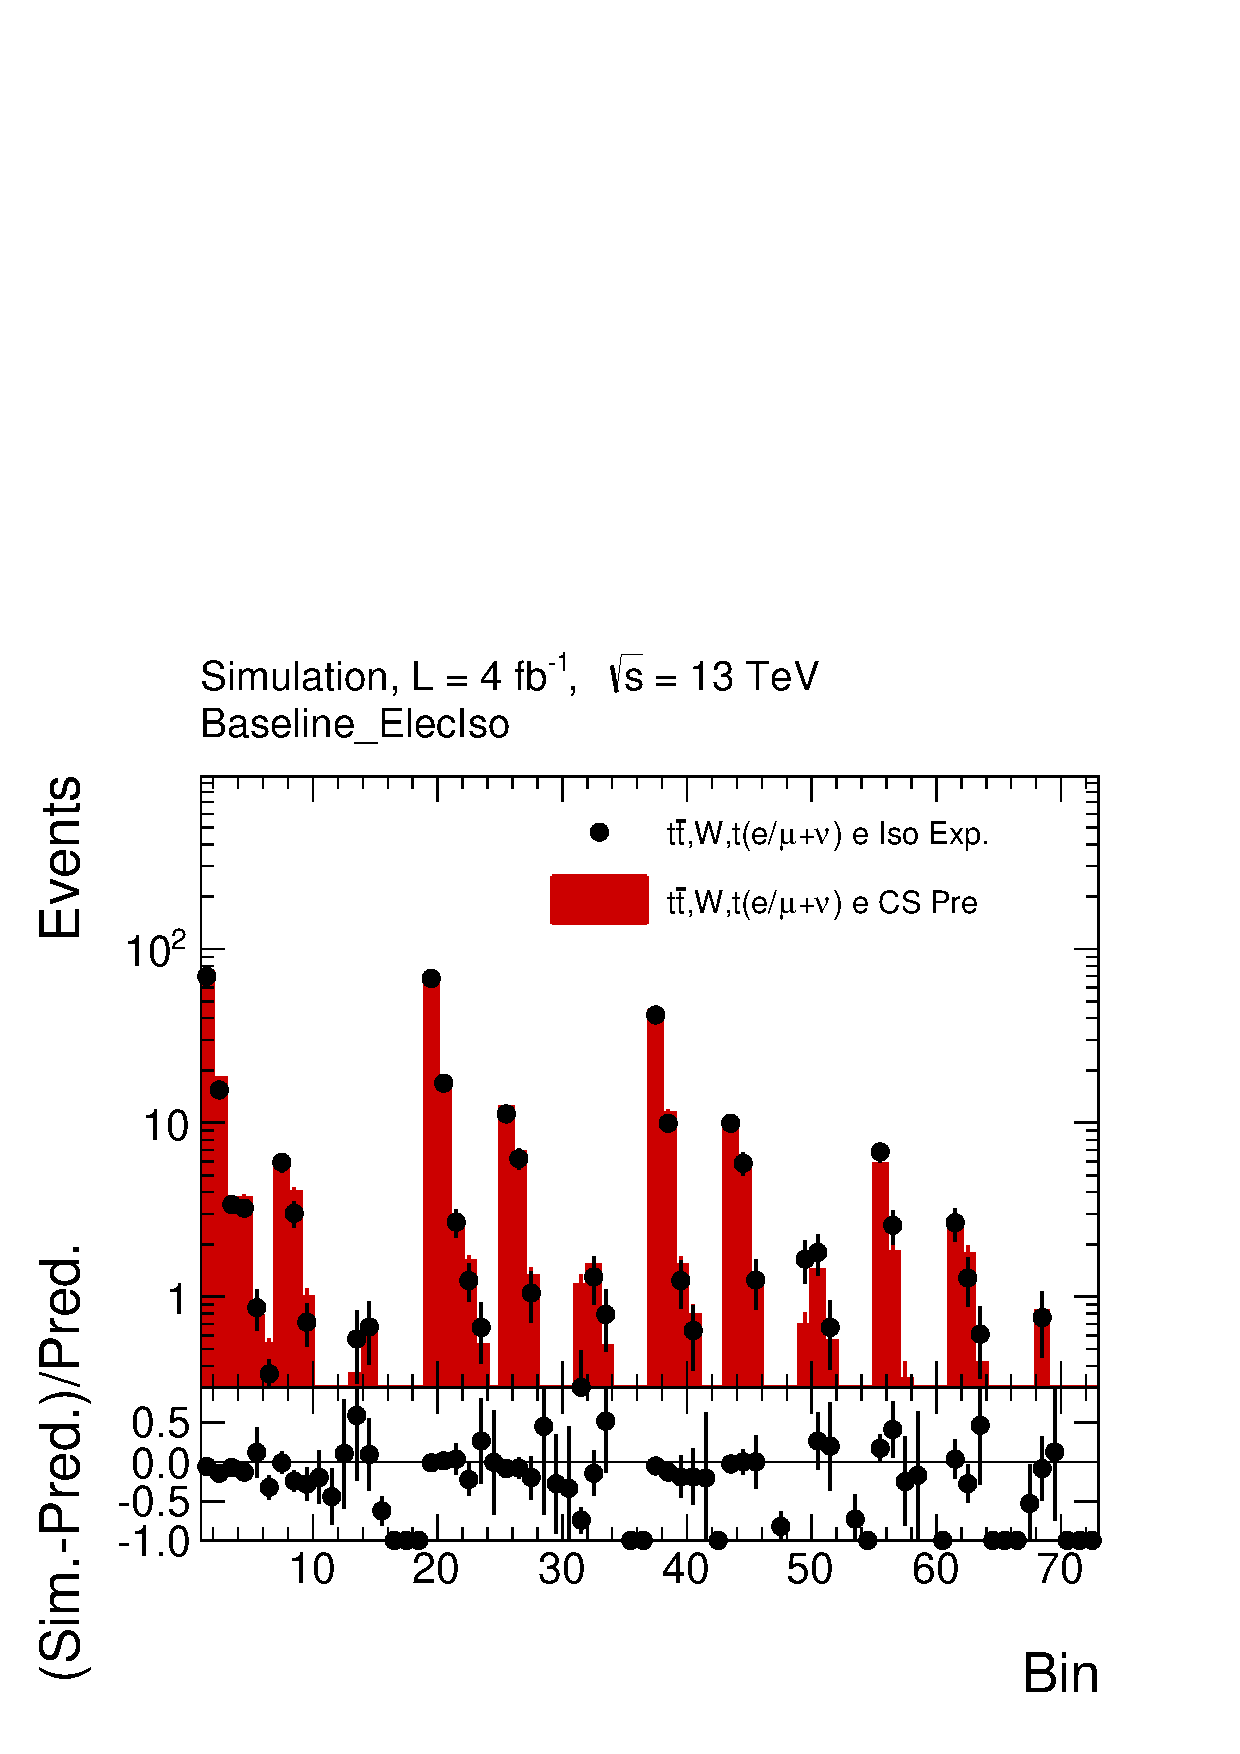
\includegraphics[width=0.90\textwidth]{figures/lost-lepton/Closure_Step_By_Step_Elec/Baseline_ElecIso/Closure_Step_By_Step_Elec__Bin__MCEx_vs_ElecCSMTWDiLepCorrected__Baseline_ElecIso.pdf}};
    \begin{scope}[x={(image.south east)},y={(image.north west)}]
%         \draw[red,ultra thick,rounded corners] (0.62,0.65) rectangle (0.78,0.75);
%         \draw[red,ultra thick,rounded corners] (0.60,0.01) rectangle (0.75,0.99); % coordinates unten links(x,y) oben rechts(x,y)
%             \draw[blue,ultra thick,rounded corners] (0.40,0.01) rectangle (0.55,0.99); % coordinates unten links(x,y) oben rechts(x,y)
    \end{scope}
\end{tikzpicture}  
       \end{center}
   \end{column}
\end{columns}
 \begin{itemize}
 \item Closure test: Non-isolated e bkg events only vs data-driven prediction using activity \& lep. \pt eff. parametrization (\HT,\NJets in backup)
 \item Good closure can be observed!
 \end{itemize}
\end{frame}


\begin{frame}
 \frametitle{Closure Test: Non-Isolated $\mu$}
   \begin{columns}
       \begin{column}{0.50\textwidth}
       \begin{center}
       \small \NJets binned isolation eff.
     \begin{tikzpicture}
    \node[anchor=south west,inner sep=0] (image) at (0,0) {\includegraphics[width=0.90\textwidth]{figures/lost-lepton/Closure_Step_By_Step_Mu/Baseline_MuIso_NJetsEff/Closure_Step_By_Step_Mu__Bin__MCEx_vs_MuCSMTWDiLepCorrected__Baseline_MuIso_NJetsEff.pdf}};
    \begin{scope}[x={(image.south east)},y={(image.north west)}]
%         \draw[red,ultra thick,rounded corners] (0.62,0.65) rectangle (0.78,0.75);
%         \draw[red,ultra thick,rounded corners] (0.60,0.01) rectangle (0.75,0.99); % coordinates unten links(x,y) oben rechts(x,y)
%             \draw[blue,ultra thick,rounded corners] (0.40,0.01) rectangle (0.55,0.99); % coordinates unten links(x,y) oben rechts(x,y)
    \end{scope}
\end{tikzpicture}       
       \end{center}
   \end{column}
       \begin{column}{0.5\textwidth}
       \begin{center}
       \small \pt \& activity binned isolation eff.
\begin{tikzpicture}
    \node[anchor=south west,inner sep=0] (image) at (0,0) {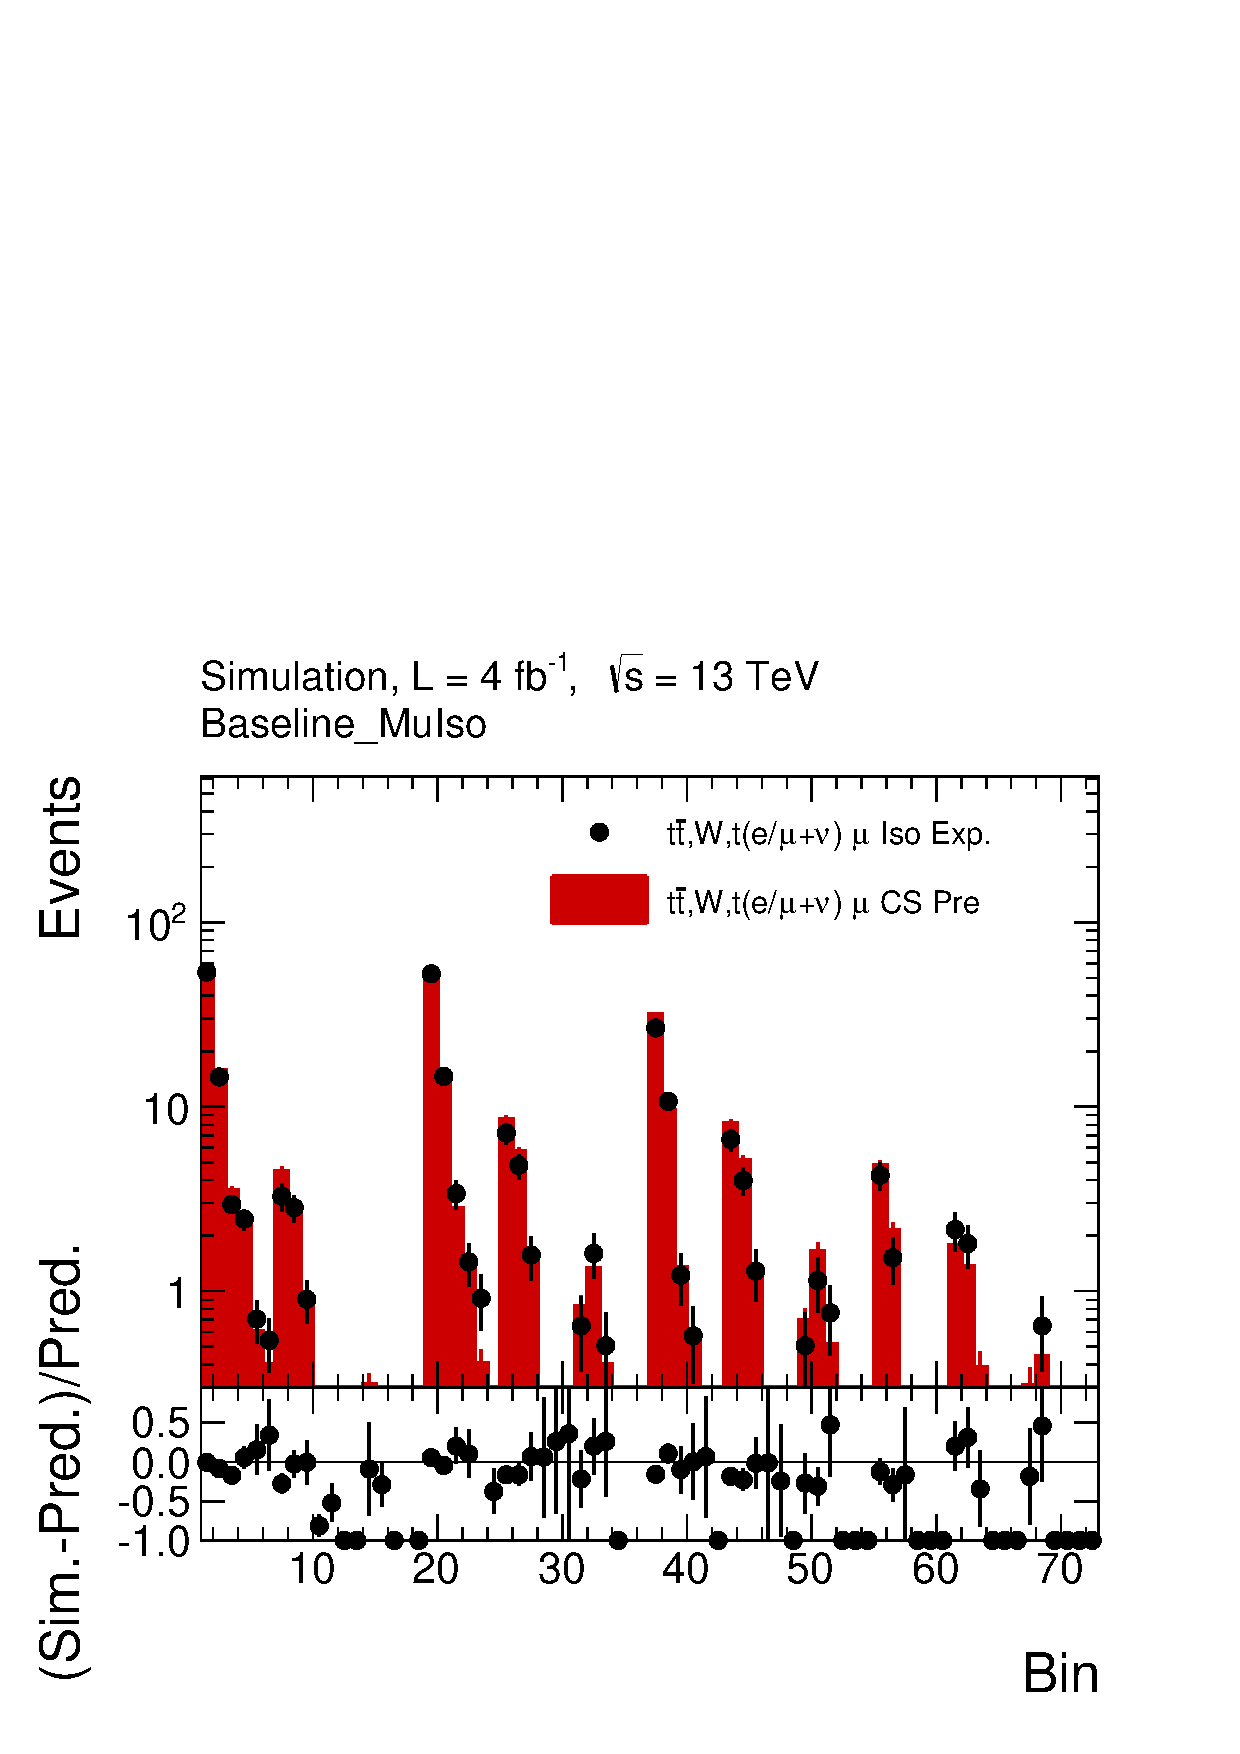
\includegraphics[width=0.90\textwidth]{figures/lost-lepton/Closure_Step_By_Step_Mu/Baseline_MuIso/Closure_Step_By_Step_Mu__Bin__MCEx_vs_MuCSMTWDiLepCorrected__Baseline_MuIso.pdf}};
    \begin{scope}[x={(image.south east)},y={(image.north west)}]
%         \draw[red,ultra thick,rounded corners] (0.62,0.65) rectangle (0.78,0.75);
%         \draw[red,ultra thick,rounded corners] (0.60,0.01) rectangle (0.75,0.99); % coordinates unten links(x,y) oben rechts(x,y)
%             \draw[blue,ultra thick,rounded corners] (0.40,0.01) rectangle (0.55,0.99); % coordinates unten links(x,y) oben rechts(x,y)
    \end{scope}
\end{tikzpicture}
       \end{center}
   \end{column}
\end{columns}
 \begin{itemize}
 \item Closure test: Non-isolated $\mu$ bkg events only vs data-driven prediction using activity \& lep. \pt \& \NJets eff. parametrization
 \end{itemize}
\end{frame}


\begin{frame}
 \frametitle{Closure Test: Non-Isolated $\mu$}
   \begin{columns}
       \begin{column}{0.50\textwidth}
       \begin{center}
       \small \HT binned isolation eff.
     \begin{tikzpicture}
    \node[anchor=south west,inner sep=0] (image) at (0,0) {\includegraphics[width=0.90\textwidth]{figures/lost-lepton/Closure_Step_By_Step_Mu/Baseline_MuIso_HTEff/Closure_Step_By_Step_Mu__Bin__MCEx_vs_MuCSMTWDiLepCorrected__Baseline_MuIso_HTEff.pdf}};
    \begin{scope}[x={(image.south east)},y={(image.north west)}]
%         \draw[red,ultra thick,rounded corners] (0.62,0.65) rectangle (0.78,0.75);
%         \draw[red,ultra thick,rounded corners] (0.60,0.01) rectangle (0.75,0.99); % coordinates unten links(x,y) oben rechts(x,y)
%             \draw[blue,ultra thick,rounded corners] (0.40,0.01) rectangle (0.55,0.99); % coordinates unten links(x,y) oben rechts(x,y)
    \end{scope}
\end{tikzpicture}       
       \end{center}
   \end{column}
       \begin{column}{0.5\textwidth}
       \begin{center}
       \small \pt \& activity binned isolation eff.
\begin{tikzpicture}
    \node[anchor=south west,inner sep=0] (image) at (0,0) {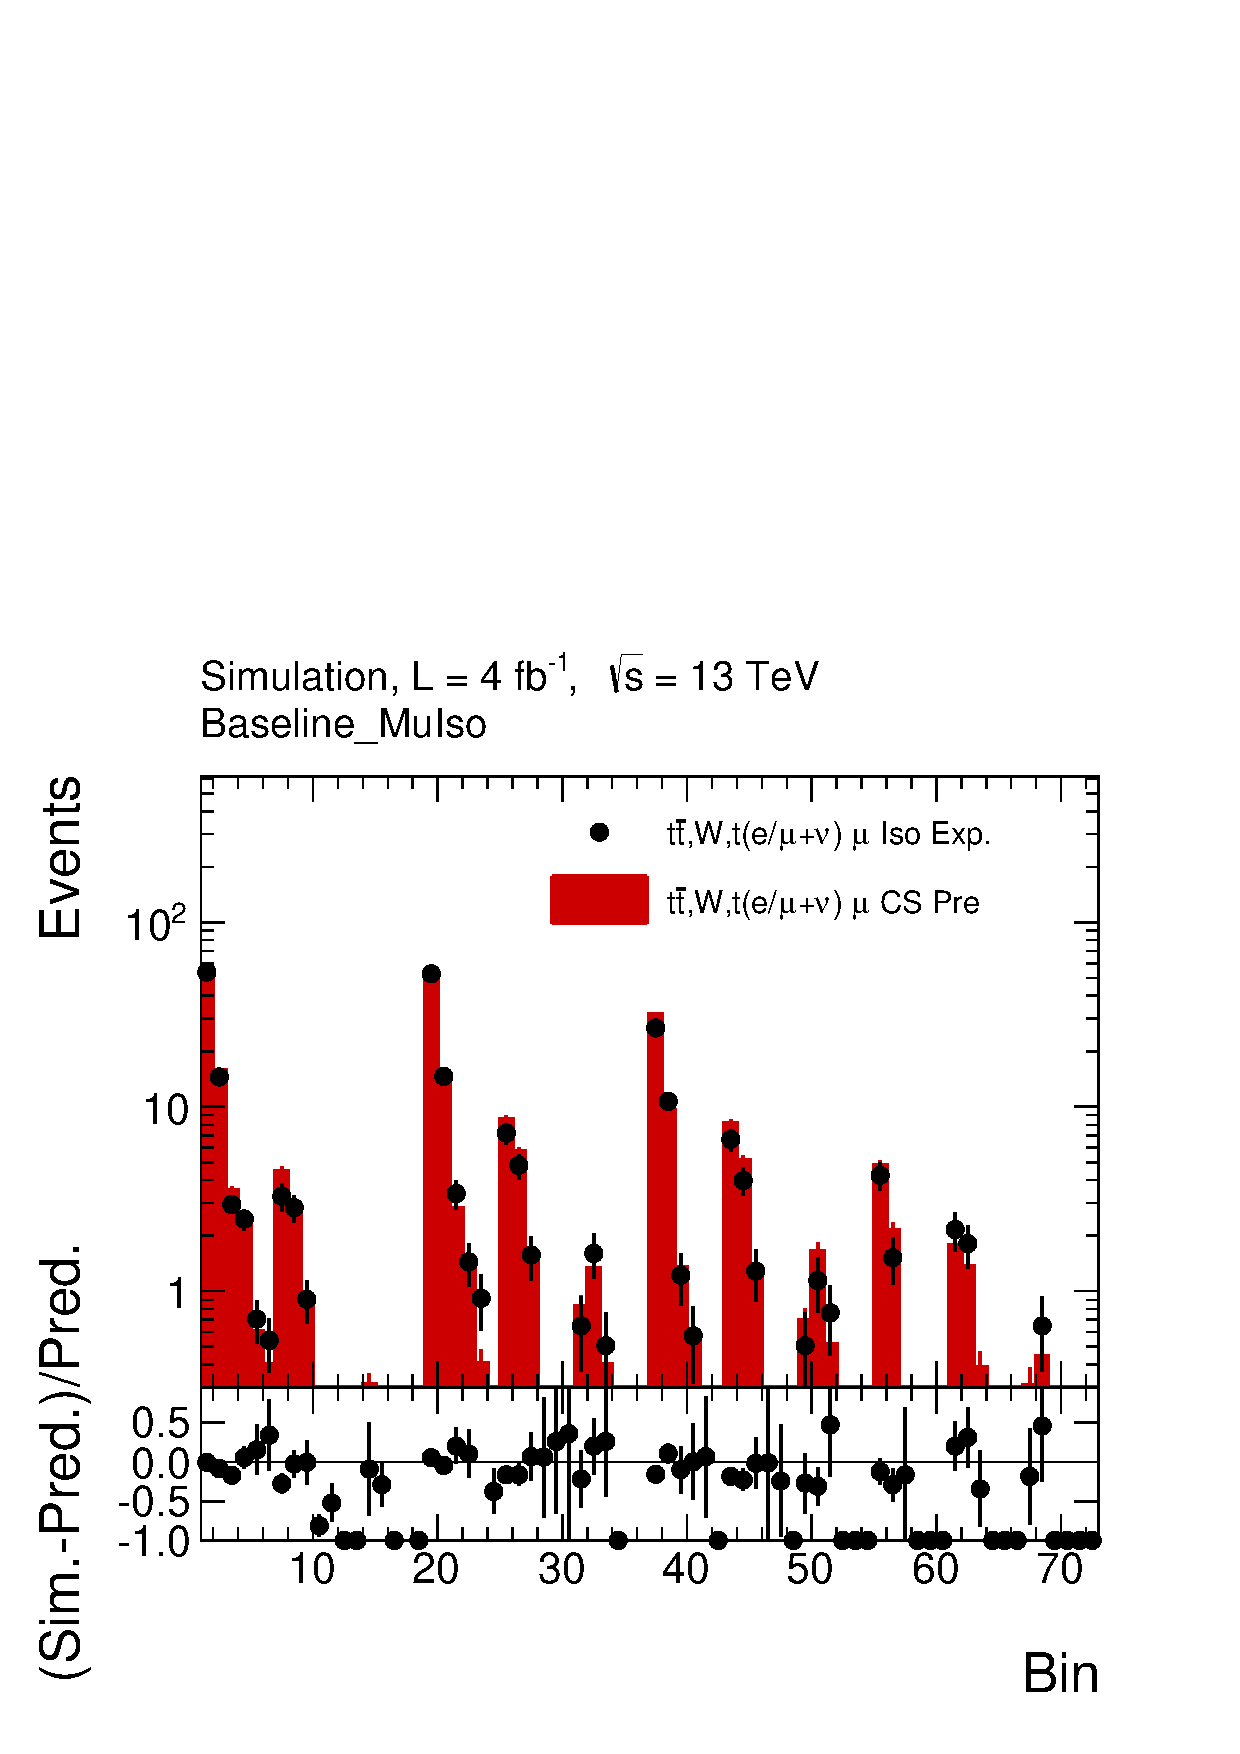
\includegraphics[width=0.90\textwidth]{figures/lost-lepton/Closure_Step_By_Step_Mu/Baseline_MuIso/Closure_Step_By_Step_Mu__Bin__MCEx_vs_MuCSMTWDiLepCorrected__Baseline_MuIso.pdf}};
    \begin{scope}[x={(image.south east)},y={(image.north west)}]
%         \draw[red,ultra thick,rounded corners] (0.62,0.65) rectangle (0.78,0.75);
%         \draw[red,ultra thick,rounded corners] (0.60,0.01) rectangle (0.75,0.99); % coordinates unten links(x,y) oben rechts(x,y)
%             \draw[blue,ultra thick,rounded corners] (0.40,0.01) rectangle (0.55,0.99); % coordinates unten links(x,y) oben rechts(x,y)
    \end{scope}
\end{tikzpicture}
       \end{center}
   \end{column}
\end{columns}
 \begin{itemize}
 \item Closure test: Non-isolated $\mu$ bkg events only vs data-driven prediction using activity \& lep. \pt (right) and \HT (left) parametrization efficiencies
 \end{itemize}
\end{frame}


\begin{frame}
 \frametitle{Closure Test: Non-Isolated e}
   \begin{columns}
       \begin{column}{0.50\textwidth}
       \begin{center}
       \small \NJets binned isolation eff.
     \begin{tikzpicture}
    \node[anchor=south west,inner sep=0] (image) at (0,0) {\includegraphics[width=0.90\textwidth]{figures/lost-lepton/Closure_Step_By_Step_Elec/Baseline_ElecIso_NJetsEff/Closure_Step_By_Step_Elec__Bin__MCEx_vs_ElecCSMTWDiLepCorrected__Baseline_ElecIso_NJetsEff.pdf}};
    \begin{scope}[x={(image.south east)},y={(image.north west)}]
%         \draw[red,ultra thick,rounded corners] (0.62,0.65) rectangle (0.78,0.75);
%         \draw[red,ultra thick,rounded corners] (0.60,0.01) rectangle (0.75,0.99); % coordinates unten links(x,y) oben rechts(x,y)
%             \draw[blue,ultra thick,rounded corners] (0.40,0.01) rectangle (0.55,0.99); % coordinates unten links(x,y) oben rechts(x,y)
    \end{scope}
\end{tikzpicture}       
       \end{center}
   \end{column}
       \begin{column}{0.5\textwidth}
       \begin{center}
       \small \pt \& activity binned isolation eff.
\begin{tikzpicture}
    \node[anchor=south west,inner sep=0] (image) at (0,0) {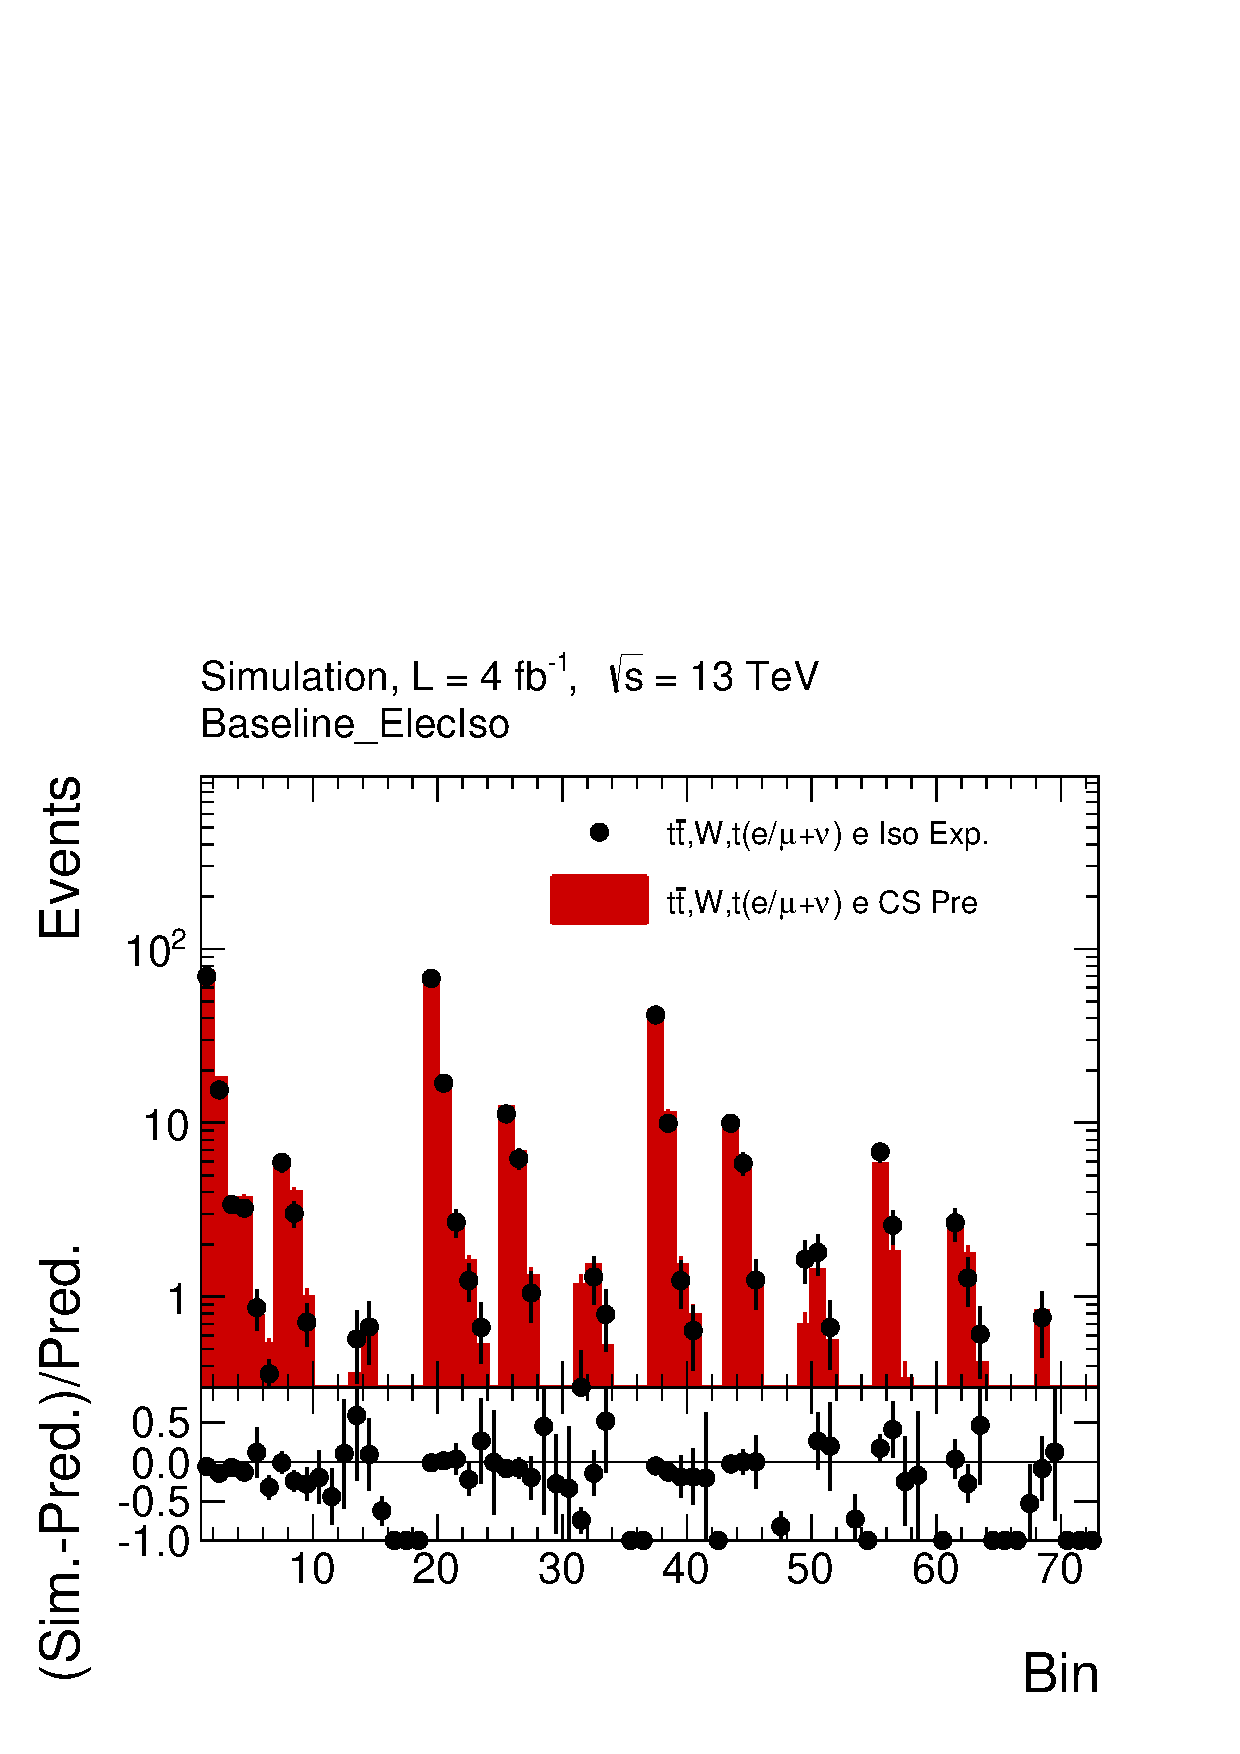
\includegraphics[width=0.90\textwidth]{figures/lost-lepton/Closure_Step_By_Step_Elec/Baseline_ElecIso/Closure_Step_By_Step_Elec__Bin__MCEx_vs_ElecCSMTWDiLepCorrected__Baseline_ElecIso.pdf}};
    \begin{scope}[x={(image.south east)},y={(image.north west)}]
%         \draw[red,ultra thick,rounded corners] (0.62,0.65) rectangle (0.78,0.75);
%         \draw[red,ultra thick,rounded corners] (0.60,0.01) rectangle (0.75,0.99); % coordinates unten links(x,y) oben rechts(x,y)
%             \draw[blue,ultra thick,rounded corners] (0.40,0.01) rectangle (0.55,0.99); % coordinates unten links(x,y) oben rechts(x,y)
    \end{scope}
\end{tikzpicture}
       \end{center}
   \end{column}
\end{columns}
 \begin{itemize}
 \item Closure test: Non-isolated e bkg events only vs data-driven prediction using activity \& lep. \pt \& \NJets eff. parametrization
 \end{itemize}
\end{frame}


\begin{frame}
 \frametitle{Closure Test: Non-Isolated e}
   \begin{columns}
       \begin{column}{0.50\textwidth}
       \begin{center}
       \small \HT binned isolation eff.
     \begin{tikzpicture}
    \node[anchor=south west,inner sep=0] (image) at (0,0) {\includegraphics[width=0.90\textwidth]{figures/lost-lepton/Closure_Step_By_Step_Elec/Baseline_ElecIso_HTEff/Closure_Step_By_Step_Elec__Bin__MCEx_vs_ElecCSMTWDiLepCorrected__Baseline_ElecIso_HTEff.pdf}};
    \begin{scope}[x={(image.south east)},y={(image.north west)}]
%         \draw[red,ultra thick,rounded corners] (0.62,0.65) rectangle (0.78,0.75);
%         \draw[red,ultra thick,rounded corners] (0.60,0.01) rectangle (0.75,0.99); % coordinates unten links(x,y) oben rechts(x,y)
%             \draw[blue,ultra thick,rounded corners] (0.40,0.01) rectangle (0.55,0.99); % coordinates unten links(x,y) oben rechts(x,y)
    \end{scope}
\end{tikzpicture}       
       \end{center}
   \end{column}
       \begin{column}{0.5\textwidth}
       \begin{center}
       \small \pt \& activity binned isolation eff.
\begin{tikzpicture}
    \node[anchor=south west,inner sep=0] (image) at (0,0) {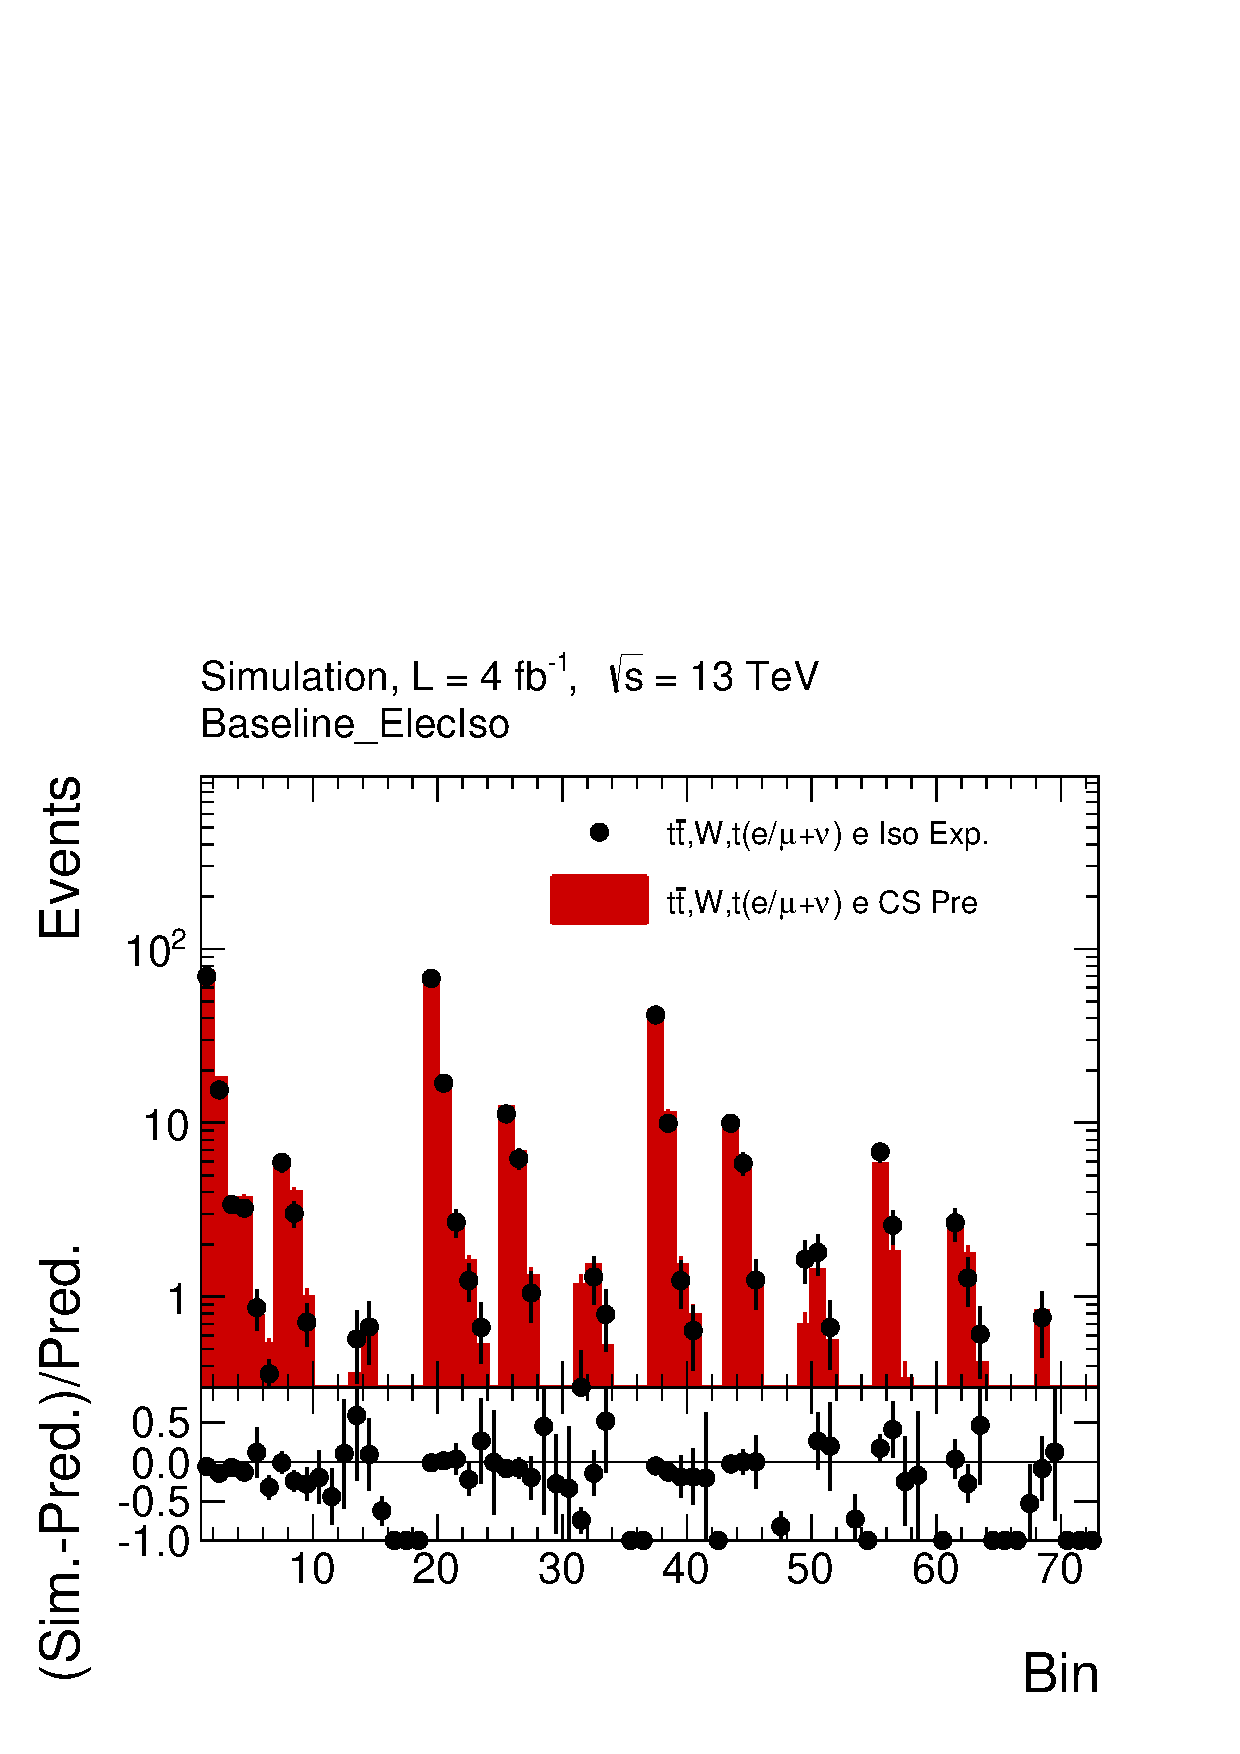
\includegraphics[width=0.90\textwidth]{figures/lost-lepton/Closure_Step_By_Step_Elec/Baseline_ElecIso/Closure_Step_By_Step_Elec__Bin__MCEx_vs_ElecCSMTWDiLepCorrected__Baseline_ElecIso.pdf}};
    \begin{scope}[x={(image.south east)},y={(image.north west)}]
%         \draw[red,ultra thick,rounded corners] (0.62,0.65) rectangle (0.78,0.75);
%         \draw[red,ultra thick,rounded corners] (0.60,0.01) rectangle (0.75,0.99); % coordinates unten links(x,y) oben rechts(x,y)
%             \draw[blue,ultra thick,rounded corners] (0.40,0.01) rectangle (0.55,0.99); % coordinates unten links(x,y) oben rechts(x,y)
    \end{scope}
\end{tikzpicture}
       \end{center}
   \end{column}
\end{columns}
 \begin{itemize}
 \item Closure test: Non-isolated e bkg events only vs data-driven prediction using activity \& lep. \pt (right) and \HT (left) parametrization efficiencies
 \end{itemize}
\end{frame}

\begin{frame}
 \frametitle{$\mu$ Iso Eff. Compare}
 \begin{columns}
  \begin{column}{0.5\textwidth}
    \centering
     \small \ttbar \& \wpj\\
    \begin{overpic}[width=.7\textwidth]{figures/efficiencies/ttbar-wpj/MuIsoHT1D.pdf}
    \end{overpic}\\
    \centering
%     \small $\Delta R$ \& lepton \pt / jet \pt
    \begin{overpic}[width=.7\textwidth]{figures/efficiencies/ttbar-wpj/MuIsoNJets1D.pdf}
    \end{overpic}   
  \end{column}
  \begin{column}{0.5\textwidth}
    \centering
    \small Tag\&Probe\\
    \begin{overpic}[width=.7\textwidth]{figures/efficiencies/tagandprobe/MuIsoHT.pdf}
    \end{overpic}\\  
    \centering
%     \small $\Delta R$ \& lepton \pt / jet \pt
    \begin{overpic}[width=.7\textwidth]{figures/efficiencies/tagandprobe/MuIsoNJets.pdf}
    \end{overpic}
  \end{column}
 \end{columns}
\end{frame}


\begin{frame}
 \frametitle{e Iso Eff. Compare}
 \begin{columns}
  \begin{column}{0.5\textwidth}
    \centering
     \small \ttbar \& \wpj\\
    \begin{overpic}[width=.7\textwidth]{figures/efficiencies/ttbar-wpj/ElecIsoHT1D.pdf}
    \end{overpic}\\
    \centering
%     \small $\Delta R$ \& lepton \pt / jet \pt
    \begin{overpic}[width=.7\textwidth]{figures/efficiencies/ttbar-wpj/ElecIsoNJets1D.pdf}
    \end{overpic}   
  \end{column}
  \begin{column}{0.5\textwidth}
    \centering
    \small Tag\&Probe\\
    \begin{overpic}[width=.7\textwidth]{figures/efficiencies/tagandprobe/ElecIsoHT.pdf}
    \end{overpic}\\  
    \centering
%     \small $\Delta R$ \& lepton \pt / jet \pt
    \begin{overpic}[width=.7\textwidth]{figures/efficiencies/tagandprobe/ElecIsoNJets.pdf}
    \end{overpic}
  \end{column}
 \end{columns}
\end{frame}

%%% Closure test
\begin{frame}
 \frametitle{Full Closure Test}
 \begin{columns}
  \begin{column}{0.5\textwidth}
    \centering
%     \small $\Delta R$ \& lepton \pt / jet \pt
    \begin{overpic}[width=.7\textwidth]{figures/lost-lepton/Closure/Baseline/Closure__HT__MCEx_vs_MuPrMTWDiLepIsoTrackReduced+ElecPrMTWDiLepIsoTrackReduced__Baseline.pdf}
    \end{overpic}\\
    \centering
%     \small $\Delta R$ \& lepton \pt / jet \pt
    \begin{overpic}[width=.7\textwidth]{figures/lost-lepton/Closure/Baseline/Closure__MHT__MCEx_vs_MuPrMTWDiLepIsoTrackReduced+ElecPrMTWDiLepIsoTrackReduced__Baseline.pdf}
    \end{overpic}   
  \end{column}
  \begin{column}{0.5\textwidth}
    \centering
%     \small $\Delta R$ \& lepton \pt / jet \pt
    \begin{overpic}[width=.7\textwidth]{figures/lost-lepton/Closure/Baseline/Closure__NJets__MCEx_vs_MuPrMTWDiLepIsoTrackReduced+ElecPrMTWDiLepIsoTrackReduced__Baseline.pdf}
    \end{overpic}\\  
    \centering
%     \small $\Delta R$ \& lepton \pt / jet \pt
    \begin{overpic}[width=.7\textwidth]{figures/lost-lepton/Closure/Baseline/Closure__BTags__MCEx_vs_MuPrMTWDiLepIsoTrackReduced+ElecPrMTWDiLepIsoTrackReduced__Baseline.pdf}
    \end{overpic}
  \end{column}
 \end{columns}
\end{frame}
\begin{frame}
 \frametitle{Full Closure Test}
    \centering
%     \small $\Delta R$ \& lepton \pt / jet \pt
    \begin{overpic}[width=.7\textwidth]{figures/lost-lepton/Closure/Baseline/Closure__Bin__MCEx_vs_MuPrMTWDiLepIsoTrackReduced+ElecPrMTWDiLepIsoTrackReduced__Baseline.pdf}
    \end{overpic}\\
\end{frame}


\begin{frame}
 \frametitle{Iso Track Reduction}
 \begin{columns}
  \begin{column}{0.5\textwidth}
    \centering
%     \small $\Delta R$ \& lepton \pt / jet \pt
    \begin{overpic}[width=.7\textwidth]{figures/lost-lepton/Closure/Baseline/Closure__HT__MCExIsoTrack_vs_MuPrMTWDiLepIsoTrackReduction+ElecPrMTWDiLepIsoTrackReduction__Baseline.pdf}
    \end{overpic}\\
    \centering
%     \small $\Delta R$ \& lepton \pt / jet \pt
    \begin{overpic}[width=.7\textwidth]{figures/lost-lepton/Closure/Baseline/Closure__MHT__MCExIsoTrack_vs_MuPrMTWDiLepIsoTrackReduction+ElecPrMTWDiLepIsoTrackReduction__Baseline.pdf}
    \end{overpic}   
  \end{column}
  \begin{column}{0.5\textwidth}
    \centering
%     \small $\Delta R$ \& lepton \pt / jet \pt
    \begin{overpic}[width=.7\textwidth]{figures/lost-lepton/Closure/Baseline/Closure__NJets__MCExIsoTrack_vs_MuPrMTWDiLepIsoTrackReduction+ElecPrMTWDiLepIsoTrackReduction__Baseline.pdf}
    \end{overpic}\\  
    \centering
%     \small $\Delta R$ \& lepton \pt / jet \pt
    \begin{overpic}[width=.7\textwidth]{figures/lost-lepton/Closure/Baseline/Closure__BTags__MCExIsoTrack_vs_MuPrMTWDiLepIsoTrackReduction+ElecPrMTWDiLepIsoTrackReduction__Baseline.pdf}
    \end{overpic}
  \end{column}
 \end{columns}
\end{frame}
\begin{frame}
 \frametitle{Iso Track Reduction}
    \centering
%     \small $\Delta R$ \& lepton \pt / jet \pt
    \begin{overpic}[width=.7\textwidth]{figures/lost-lepton/Closure/Baseline/Closure__Bin__MCExIsoTrack_vs_MuPrMTWDiLepIsoTrackReduction+ElecPrMTWDiLepIsoTrackReduction__Baseline.pdf}
    \end{overpic}\\
\end{frame}


% \begin{frame}
%  \frametitle{Include}
%  \begin{itemize}
%   \item Closure overall
%   \item Iso reco acc separated
%   \item Closure iso track contribution
%   \item Efficiencies
%   \item All lost-lepton sketches
%  \end{itemize}
% 
% \end{frame}





\begin{frame}
\frametitle{Concept: Estimating Lost $e,\mu$ from \wpj \& \ttbar Events}
 \begin{center}
\begin{tikzpicture}
    \node[anchor=south west,inner sep=0] (image) at (0,0) {\includegraphics[width=0.75\textwidth]{figures/Sketches/LostLeptonSketch_mu_pred_full.pdf}};
    \begin{scope}[x={(image.south east)},y={(image.north west)}]
%         \draw[red,ultra thick,rounded corners] (0.62,0.65) rectangle (0.78,0.75);
%         \draw[red,ultra thick,rounded corners] (0.60,0.01) rectangle (0.75,0.99); % coordinates unten links(x,y) oben rechts(x,y)
%             \draw[blue,ultra thick,rounded corners] (0.40,0.01) rectangle (0.55,0.99); % coordinates unten links(x,y) oben rechts(x,y)
    \end{scope}
\end{tikzpicture}
 \end{center}
\end{frame}

\begin{frame}
 \frametitle{Reconstruction \& ID validation}
 
   \begin{columns}
 \begin{column}{0.50\textwidth}
 
   \begin{itemize}
  \item We compute our combined reco/ID eff using gen information:
  \begin{itemize}
   \item Reco/ID Eff.: Select events with prompt lepton $\rightarrow$ Ask for $\pt>10\gev$ \& $|\eta|<2.5(2.4)$ (on gen) $\rightarrow$ try to match well reconstructed and ID lepton (on reco level) $eff.=p/(p+f)$
  \end{itemize}
  \item Tag\&Probe Difficulty:
  \item No gen info available. Test object selected on reco level. Most basic object desirable (avoid gab see above).
  \end{itemize}
 \end{column}
  \begin{column}{0.50\textwidth}
\begin{tikzpicture}
    \node[anchor=south west,inner sep=0] (image) at (0,0) {\includegraphics[width=1.\textwidth]{figures/efficiencies/tagandprobe/MuRecoPFCandProbeNoFailPeak.pdf}};
    \begin{scope}[x={(image.south east)},y={(image.north west)}]
%         \draw[red,ultra thick,rounded corners] (0.62,0.65) rectangle (0.78,0.75);
    \end{scope}
\end{tikzpicture}  
\begin{itemize}
 \item BUT need to keep ratio Z mass signal over bkg reasonable for fit! Especially in failing collection!
 \item $Eff. = p / (p + f)$  
\end{itemize}
  \end{column}
 \end{columns}
\end{frame}
\begin{frame}
 \frametitle{Reconstruction \& ID Tag\&Probe Setup}
 
 Setup:
 \begin{itemize}
  \item Tag: Isolated $\mu/e$
  \item Probe:
  \begin{itemize}
   \item $\mu$: miniAOD slimmedMuon; Gap: Missing muons within acceptance ($\pt>10\gev$ \& $|\eta|<2.4$)  that are NOT slimmedMuons\\ (most basic: tracker muons)
   \item $e$: miniAOD slimmedPhoton; Gap: Missing electrons within acceptance ($\pt>10\gev$ \& $|\eta|<2.5$) that are NOT Photons (especially in high activity region) (most basic: superclusters)
  \end{itemize}
 \end{itemize}
\end{frame}
\begin{frame}
 \frametitle{$\mu$ Reconstruction/ID Efficiencies}
  \begin{columns}

   \begin{column}{0.33\textwidth}
     \begin{itemize}
   \item $\mu$ Reco/ID \ttbar \& \wpj eff.
  \end{itemize}
    \begin{tikzpicture}
    \node[anchor=south west,inner sep=0] (image) at (0,0) {\includegraphics[width=1.\textwidth]{figures/efficiencies/MuRecoPTActivity.pdf}};
    \begin{scope}[x={(image.south east)},y={(image.north west)}]
%         \draw[red,ultra thick,rounded corners] (0.62,0.65) rectangle (0.78,0.75);
%         \draw[red,ultra thick,rounded corners] (0.60,0.01) rectangle (0.75,0.99); % cordinates unten links(x,y) oben rechts(x,y)
    \end{scope}
   \end{tikzpicture}
   \end{column}
   \begin{column}{0.33\textwidth}
   \begin{itemize}
    \item $\mu$ Reco/ID Tag \& Probe eff.
   \end{itemize}

    \begin{tikzpicture}
    \node[anchor=south west,inner sep=0] (image) at (0,0) {\includegraphics[width=1.\textwidth]{figures/efficiencies/MuRecoTagAndProbeMC.pdf}};
    \begin{scope}[x={(image.south east)},y={(image.north west)}]
%         \draw[red,ultra thick,rounded corners] (0.62,0.65) rectangle (0.78,0.75);
%         \draw[red,ultra thick,rounded corners] (0.60,0.01) rectangle (0.75,0.99); % cordinates unten links(x,y) oben rechts(x,y)
    \end{scope}
   \end{tikzpicture}
   \end{column}
   \begin{column}{0.33\textwidth}
   \begin{itemize}
    \item Ratio: \ttbar \& \wpj / Tag \& Probe eff.
   \end{itemize}

    \begin{tikzpicture}
    \node[anchor=south west,inner sep=0] (image) at (0,0) {\includegraphics[width=1.\textwidth]{figures/efficiencies/MuRecoPTActivity_ratio.pdf}};
    \begin{scope}[x={(image.south east)},y={(image.north west)}]
%         \draw[red,ultra thick,rounded corners] (0.62,0.65) rectangle (0.78,0.75);
%         \draw[red,ultra thick,rounded corners] (0.60,0.01) rectangle (0.75,0.99); % cordinates unten links(x,y) oben rechts(x,y)
    \end{scope}
   \end{tikzpicture}
   \end{column}
  \end{columns}
\begin{itemize}
 \item Overall the expected higher efficiencies can be observed in Tag\&Probe due to the gab of probe object (slimmedMuon) and all muons within acceptance
\end{itemize}

\end{frame}


\begin{frame}
 \frametitle{e Reconstruction/ID Efficiencies}
  \begin{columns}

   \begin{column}{0.33\textwidth}
     \begin{itemize}
   \item e Reco/ID \ttbar \& \wpj eff.
  \end{itemize}
    \begin{tikzpicture}
    \node[anchor=south west,inner sep=0] (image) at (0,0) {\includegraphics[width=1.\textwidth]{figures/efficiencies/ElecRecoPTActivity.pdf}};
    \begin{scope}[x={(image.south east)},y={(image.north west)}]
%         \draw[red,ultra thick,rounded corners] (0.62,0.65) rectangle (0.78,0.75);
%         \draw[red,ultra thick,rounded corners] (0.60,0.01) rectangle (0.75,0.99); % cordinates unten links(x,y) oben rechts(x,y)
    \end{scope}
   \end{tikzpicture}
   \end{column}
   \begin{column}{0.33\textwidth}
   \begin{itemize}
    \item e Reco/ID Tag \& Probe eff.
   \end{itemize}

    \begin{tikzpicture}
    \node[anchor=south west,inner sep=0] (image) at (0,0) {\includegraphics[width=1.\textwidth]{figures/efficiencies/ElecRecoTagAndProbeMC.pdf}};
    \begin{scope}[x={(image.south east)},y={(image.north west)}]
%         \draw[red,ultra thick,rounded corners] (0.62,0.65) rectangle (0.78,0.75);
%         \draw[red,ultra thick,rounded corners] (0.60,0.01) rectangle (0.75,0.99); % cordinates unten links(x,y) oben rechts(x,y)
    \end{scope}
   \end{tikzpicture}
   \end{column}
   \begin{column}{0.33\textwidth}
   \begin{itemize}
    \item Ratio: \ttbar \& \wpj / Tag \& Probe eff.
   \end{itemize}

    \begin{tikzpicture}
    \node[anchor=south west,inner sep=0] (image) at (0,0) {\includegraphics[width=1.\textwidth]{figures/efficiencies/ElecRecoPTActivity_ratio.pdf}};
    \begin{scope}[x={(image.south east)},y={(image.north west)}]
%         \draw[red,ultra thick,rounded corners] (0.62,0.65) rectangle (0.78,0.75);
%         \draw[red,ultra thick,rounded corners] (0.60,0.01) rectangle (0.75,0.99); % cordinates unten links(x,y) oben rechts(x,y)
    \end{scope}
   \end{tikzpicture}
   \end{column}
  \end{columns}
\begin{itemize}
 \item At high $\pt$ to activity ratio good agreement. Increasing activity increases probability to lose already probe object (photon) biases to higher eff in Tag\&Probe. Also $\pt$ threshold of Probe objects at 15\gev.
\end{itemize}

\end{frame}


\begin{frame}
 \frametitle{Isolation Efficiencies}
 \begin{columns}
  \begin{column}{0.5\textwidth}
    \centering
%     \small $\Delta R$ \& lepton \pt / jet \pt
    \begin{overpic}[width=.7\textwidth]{figures/lost-lepton/Closure/Baseline/Closure__HT__MCExIsoTrack_vs_MuPrMTWDiLepIsoTrackReduction+ElecPrMTWDiLepIsoTrackReduction__Baseline.pdf}
    \end{overpic}\\
    \centering
%     \small $\Delta R$ \& lepton \pt / jet \pt
    \begin{overpic}[width=.7\textwidth]{figures/lost-lepton/Closure/Baseline/Closure__MHT__MCExIsoTrack_vs_MuPrMTWDiLepIsoTrackReduction+ElecPrMTWDiLepIsoTrackReduction__Baseline.pdf}
    \end{overpic}   
  \end{column}
  \begin{column}{0.5\textwidth}
    \centering
%     \small $\Delta R$ \& lepton \pt / jet \pt
    \begin{overpic}[width=.7\textwidth]{figures/lost-lepton/Closure/Baseline/Closure__NJets__MCExIsoTrack_vs_MuPrMTWDiLepIsoTrackReduction+ElecPrMTWDiLepIsoTrackReduction__Baseline.pdf}
    \end{overpic}\\  
    \centering
%     \small $\Delta R$ \& lepton \pt / jet \pt
    \begin{overpic}[width=.7\textwidth]{figures/lost-lepton/Closure/Baseline/Closure__BTags__MCExIsoTrack_vs_MuPrMTWDiLepIsoTrackReduction+ElecPrMTWDiLepIsoTrackReduction__Baseline.pdf}
    \end{overpic}
  \end{column}
 \end{columns}
\end{frame}

% --------------------------------------------------

\setcounter{framenumber}{20}

\end{document}

